\documentclass[english,twoside,openright]{UH_DS_MSc}

\usepackage{lmodern}
\usepackage{textcomp}
\usepackage[pdftex]{color, graphicx}
\usepackage[pdftex, plainpages=false]{hyperref}
\usepackage{fancyhdr}
\usepackage{amsmath, amssymb}
\usepackage[footnotesize,bf]{caption}
\usepackage{blindtext}
\usepackage{titlesec}
\usepackage[titletoc]{appendix}
\usepackage{hyperref}
\usepackage[nodayofweek,level]{datetime}
\newcommand{\thesisdate}{\formatdate{19}{12}{2024}}
\usepackage{algorithm}
\usepackage{algpseudocode}
\usepackage{subcaption}

\onehalfspacing

\sloppy
\usepackage[dvipsnames]{xcolor}
\usepackage{tikz}
\usetikzlibrary{shapes.geometric, arrows}
\usepackage[skins]{tcolorbox}

\tikzstyle{nnmodel} = [trapezium, draw=black, fill=blue!20, trapezium left angle=120, trapezium right angle=120]
\tikzstyle{textcontainer} = [rectangle]
\tikzstyle{imageframe} = [rectangle]
\tikzstyle{arrow} = [thick, ->, >=stealth, draw=Maroon, shorten <= 2, shorten >= 2]
\tikzstyle{nonactivearrow} = [thick, ->, >=stealth, draw=Maroon!30, shorten <= 2, shorten >= 2]

\title{Fine-tuned Optical Character Recognition for Dental Fossil Markings}
\author{Riikka Korolainen}
\date{\thesisdate}
\prof{Professor Indr{\.e} \v{Z}liobait{\.e}}
\censors{Associate Professor Arto Klami}{}{}
\keywords{Optical character recognition, Transfer learning, Paleontological databases}
\depositeplace{}
\additionalinformation{Code and pre-trained models are available on \href{https://github.com/korolainenriikka/fine-tuned-ocr-for-dental-markings}{GitHub}.}


\classification{\protect{\ \\
\  Computing methodologies  $\rightarrow$  Machine learning $\rightarrow$ Machine learning approaches $\rightarrow$ Neural Networks \  \\
\  Computing methodologies $\rightarrow$ Machine learning $\rightarrow$ Learning paradigms $\rightarrow$ Multi-task learning $\rightarrow$ Transfer learning \  \\
\  Applied computing $\rightarrow$ Physical sciences and engineering $\rightarrow$ Earth and atmospheric sciences \  \\
}}

\hypersetup{
    unicode=true,
    pdftoolbar=true,
    pdfmenubar=true,
    pdffitwindow=false,
    pdfstartview={FitH},
    pdftitle={},
    pdfauthor={},
    pdfsubject={},
    pdfcreator={},
    pdfproducer={pdfLaTeX},
    pdfnewwindow=true,
    colorlinks=true,
    linkcolor=black, 
    citecolor=black,
    filecolor=magenta,
    urlcolor=cyan
}

\begin{document}

\maketitle

\begin{abstract}

Uniforming the structure of handwritten fossil catalogues maintained at natural history museums
worldwide exhibits great potential for increasing the accuracy of paleontological data analysis
by increasing sample sizes. Approximately 90 000 of such samples reside in the archives of the
National Museums of Kenya, and an ongoing effort is to store this data in a digital format for
better accessibility. A previous project utilized a commercial optical character recognition service
for the automated reading of these catalogues. This generalist handwriting detection model could not detect special characters used to denote tooth samples, leading to loss of information and
detection mistakes.
This thesis proposes a classifier chain approach for detecting which tooth is shown on an image of
a tooth marking and a pipeline for Uniforming the dental notation present in the bone or tooth
type specifying column. The best base model is searched for by comparing multiple convolutional
and transformer architectures to classify notation to upper or lower jaw, with the best validation
accuracy of 96.75\% using AlexNet. In the experiments it is found that the quality of optimum found
in training affects results significantly, leading to margins of error up to 10\% for architecture
comparisons in a small data case. The clearest result is that not freezing layers, without exception,
leads to better results. Because of this, it is theorized that the utility of transfer learning mostly
stems from being able to train more, rather than the ability to re-use a feature extractor. The
pipeline with best-performing classifiers is used to obtain an accurate reading of the catalogues
of the National Museums of Kenya, and the tool is published to be used by the paleontological
community for further digitization efforts.

\end{abstract}

\mytableofcontents

\mynomenclature

\chapter{Introduction}

The field of paleoecology conducts data analysis over the fossil record.
Such analysis is literally started from the ground: after a promising fossil site has been identified, searched, and a fossil specimen has been found, the specimen is 
carefully analyzed: which bone and species, and which time period the fragment is from. On-site, such information has historically been logged on field slips, small thin sheets of 
paper with a pre-printed form. The analysis has then been traditionally conducted by 
collecting such entries, sometimes collected in handwritten tabular catalogues, and running statistical 
tests on the sample set. With this analysis, knowledge of the distant past, such as climate, habitats, and 
vegetation can be deduced~\cite{Faith_Lyman_2019}. Syntheses of such results consequently allow us to 
answer larger questions, such as how ecosystems reacted to climate changes, how mass extinction events 
came about, and what the living world could be like~\cite{Zliobaite2023}. Understandably, answering such 
questions has become ever more pressing.

To find answers to large-scale problems, computational methods requiring large datasets have come about. Due to the infeasibility of inspecting large numbers of specimens across sometimes multiple 
continents, specimens residing in archives of institutions have been recorded to digital, public databases~\cite{uhenCardCatalogsComputers2013}.
One such institution is the National Museums of Kenya that holds a large fraction of data collected from one 
of the most valuable fossil sites globally, Lake Turkana. The sheer amount of physical samples in the museum storage
makes keeping them safe a significant challenge, a risk to global heritage now attracting attention across continents,
 as reported by the Wall Street Journal~\cite{hotzMuseumOverflowingPrehistoric2024}.
 A project digitizing the handwritten catalogues hosted by the National Museums of Kenya was started by
using commercial optical character recognition (OCR) software, Azure Vision~\cite{azurevision}, combined with heuristic and machine learning approaches, 
resulting in satisfactory accuracy on conventional handwritten text. However, this 
approach was not able to recognize special characters that denote which teeth each specimen contains. This work aims 
to continue the project by digitizing these markings accurately.

Specifically, the goal of this thesis is to recognize tooth type,
jaw, and index number markings to increase the accuracy of the element description in
the digitized fossil dataset of the National Museums of Kenya. As input data, both scan images of tabular fossil catalogues,
and outputs from Azure Vision are used.
The output consists of sentence and word-level readings, along with bounding boxes defining 
the location of each word or sentence. The main research question is the following: 

How, given scan images, bounding boxes, and generalist OCR outputs, can the accuracy of the readings of the tooth markings be improved?

This thesis proposes a univariate classifier chain for
uniforming dental notation. Each element description is processed 
word-by-word, and for each word, only those recognized as tooth markings
by using a regular expression on the Azure Vision reading are given to tooth marking
classifiers. This way, more complex cases are left unprocessed, a desirable
approach as this is one of the first works attempting automated cleaning 
of digitized fossil data. The chain consists of three classifiers: the first one detects the tooth type specifying the letter on the image, the second detects whether the tooth is from the upper or lower jaw,
and the third recognizes the index number. Finally, all these inferences are combined into tooth notation and concatenated to a corrected element 
description. 

In the experiments for building the univariate classifiers, various base models and training configurations are compared.
AlexNet with no layer freezing is found to result in the best test accuracy of 92.31\% on the 
upper or lower jaw classification task, however, it is found that different hyperparameter 
configurations influence the scores by up to 10\%. 
Fractions of test images classified correctly with above-99.7\% confidence are 
counted to estimate the amount of saved manual verifying effort, these scores ranging 
from 58\% to 94.5\% depending on the classification task.
The approach of annotating a dental marking with the minimum 
confidence of all classifiers causes most of the final confidence scores 
to be too low to bypass manual verifying, and therefore little manual labor may be 
saved with this initial solution. Still, it is proven that the proposed approach works and that 
accurate classifiers with test accuracies ranging from 88.0\% to 100.0\% can be built 
with the techniques presented.

The direct impact of this work is an improved precision of the tooth element entries in the digitized 
fossil catalogues of the National Museums of Kenya, but the results apply to a wider domain.
Intuitively, the results are directly applicable to other fossil archives using similar notation: only a fine-tuning of the 
models to the data is necessary.
For other handwritten archives, the results presented can be used to improve recognition accuracy, especially when the target character set can be expressed with multivariate output data. This could, for 
instance, be handwriting with occasional underlinings, where the bivariate output could be the letter and a boolean variable for if underlining was detected.

The rest of this thesis is organized as follows. First, the necessary background theory is 
presented. For paleoecology, the background covers 
foundational ecological theory followed by a brief introduction to methods used in
paleoenvironmental reconstruction, especially focusing on inferences from tooth data. This is
followed by a presentation of the mammal tooth row.
For deep neural networks, the following concepts are introduced:
The basic network structure, how training is conducted, building blocks of character-recognizing network architectures, and transfer learning. 
Second, related work is presented, both on
handwritten archive digitization and transfer learning with character-recognizing models.
Next, the experimental setup is introduced, covering dataset creation, labeling, and data 
preprocessing, followed by base model and transfer learning method selection. After this, 
the results of the experiments are presented and discussed. Finally, the work is concluded.

\chapter{Fundamentals on Paleoecology}

Paleoecology is a field that conducts data analysis on fossil specimens. The most common type of 
this analysis is paleoenvironmental reconstruction: deducing what past habitats were like and which 
changes they have undergone~\cite{Faith_Lyman_2019_ch2}.

The high-level process for reconstructing paleoenvironments is to find a relationship between the traits of an animal or plant community in the present and use this 
relationship to estimate paleoenvironmental variables based on species found in a fossil assemblage.
Traditionally, these relationships are constructed with expert knowledge of each species: the environmental conditions of
each species are studied and limits known as tolerances are learned. These sets of tolerances form niches,
the set of possible environmental conditions a species can live in~\cite{Faith_Lyman_2019_ch2}. Finally, these insights are aggregated to 
draw conclusions on past environments based on which species occur in fossil records in a given location and time.
Naturally, there are multitudes of methods for drawing environmental conclusions from fossil data based on 
tolerances and niches, and the methods have many caveats, thoroughly surveyed by Faith and Lyman~\cite{Faith_Lyman_2019}. One of the major limitations is that with a big set of environmental signals provided by the niches of each species, drawing conclusions from multitudes of often partially conflicting signals is a challenge.

In this chapter, background on paleoenvironmental reconstruction is reviewed, focusing on methods for dental fossil data.
Section~\ref{sect:ecometrics} highlights dental ecometrics, a method for constructing mappings from dental elements to environmental traits to motivate the 
need for representative and accurate tooth fossil datasets. As further background on the data, Section~\ref{sect:mammal_teeth} presents the mammal teeth 
row along with related terminology.

\section{Dental ecometrics}
\label{sect:ecometrics}

Dental ecometrics is a method for constructing transfer functions, mappings from species occurrences to environmental traits.
These can be learned using statistical models, such as regression, or classic machine learning methods.
Using transfer functions is considered more accurate than expert analysis on tolerances and niches: the latter
can contain subjective interpretations, and transfer functions allow analyzing larger sets of species occurrences than would 
 be possible for a human analyst~\cite{Faith_Lyman_2019_ch9}.

Dental ecometrics constructs transfer functions with dental traits as input variables~\cite{Faith_Lyman_2019_ch9, oksanenHumboldtianApproachLife2019}.
The method is a subfield of ecomorphology; the study of the relation of functional traits of animals and plants with their livelihood
\cite{oksanenHumboldtianApproachLife2019}. The high-level reasoning behind the method is that teeth evolve to 
shapes that are most suitable for processing vegetation in the habitat, thus one can infer vegetation based on tooth shapes, 
which then serves as a good proxy for environmental conditions~\cite{oksanenHumboldtianApproachLife2019}. 
When the environment changes, animals have to move to habitats where the vegetation is digestible with their teeth, and therefore
analysis on environmental change can be performed even on smaller timescales than evolution would allow~\cite{fortelius}. For example, both precipitation~\cite{fortelius}
and temperature~\cite{oksanenHumboldtianApproachLife2019} can be learned based on dental lophs, number of cutting blade shapes, and hypsodonty, the height of the
molar crown, with the following analysis. One can roughly divide available plants as grass, that has more water and is easier to chew, and 
browse, drier and rougher plants. Dominant molars are primarily used to chew these plants, and it is known that to digest grass, a high 
crown is required due to tooth erosion and that to digest browse, cutting blades in teeth are required to cut the fibrous plants to pieces.
Therefore, one can find statistical relationships between these tooth measurements and environmental conditions favorable 
for the growth of grass or browse. Then, a large number of fossilized molars can be collected, the crown heights and blade shapes measured, and a dataset of 
tooth types constructed. The previously learned function can then be applied to this data set
 to estimate environmental variables. These insights on 
 past environments and how habitats interacted with their changes can 
 in turn be used to inform the present: for example, it is possible to predict how much local ground temperature rises when tree cover is lost~\cite{fortelius} and
information like this is crucial in understanding the processes occurring with climate
change.
  Again, the true relationships are much more complicated 
 than the straightforward thought process presented here, but the rough idea is accurate.

Many studies on paleoenvironmental reconstruction list data availability as one of the most major limitations~\cite{oksanenHumboldtianApproachLife2019,fortelius}.
As geological time spans are huge, studies have to 
resort to time resolutions of hundreds of thousands of years (e.g.,~\cite {fortelius}) because of a lack 
of sufficient sample sizes. One of the greatest challenges in verifying a hypothesis on 
paleoenvironments is the effort required to collect and curate a dataset; for instance, some ecometric
analysis works start by measuring the dental traits~\cite{fortelius}, an effort that could be saved 
if measurements were collected once and then stored in a structured manner. For this reason, the 
creation and maintenance of paleontological databases is of central importance. This is accentuated 
in the case of the catalogues processed in this work that store most of the fossils found from the Turkana basin: it is suspected that
important steps in human evolution occurred there, the mammal record is especially dense~\cite{fortelius}, and the area has undergone many environmental transitions in the past~\cite{Zliobaite2023}.

The goal of this work is to recognize dental markings to increase the accuracy of the element descriptions in
the digitized fossil dataset of the National Museums of Kenya,
with the primary aim that the structured, digital data would allow for 
more accurate analysis thanks to larger samples and less tedium in 
setting up experiments. The terminology special to fossils present in 
the curated data is presented next.

\section{Composition of mammal teeth}
\label{sect:mammal_teeth}

Since geological events erode fast-decomposing organic remains first, the hardest materials in 
the corpse represent most of fossil collections. These hard materials include shells, bones, and especially teeth, the last being prominent in fossil data analysis also because they encode diverse clues on 
the livelihood of the organism~\cite{Faith_Lyman_2019}.
This section presents the naming and indexing system for mammal teeth commonly used in paleontological datasets,
as described by Hillson~\cite{Hillson_2005}, and some common shorthand versions present in the dataset digitized in this work.

Specimens including fragments of the jaw are described with terminology related 
to the jaw bones. All mammals share the same bone structure around the mouth: the lower jaw consists 
of two bones called \textit{mandibles}, whereas the upper jaw consists of bones called 
\textit{maxilla} and \textit{premaxilla} that also form large parts of the face.
A common trait across many mammals is also that permanent teeth erupt in the 
youth of the animal, replacing the 'milk' or \textit{deciduous} teeth. Shorthands commonly used for these 
terms are 'mand' for mandibles and the letter 'D' for deciduous teeth.

Mammals have four tooth types: \textit{incisor}, \textit{canine}, \textit{premolar},
and \textit{molar}, and tooth positions are indexed with a numbering system. Moving from the middle of the tooth row
towards the side, there are up to three 
incisors, used for catching food and denoted with the letter 'i'. Behind them is the canine tooth, denoted with the letter 'c'. Behind the canine are typically up to four premolars, noted with 'p'. These 
teeth vary most between taxa in form with functions including cutting, holding, and chewing food.
The teeth at the back of the row are called molars, 'm', and are primarily used for chewing. Molars, like the other tooth types, 
vary in number between taxa and are typically at most three. The numbers are always increasing when moving back in the tooth row, but in
 the case of missing teeth in a taxon, the numbers do not necessarily start from one: instead, the number is chosen to 
have teeth with the same numbers as alike each other as possible. Thus, a taxon with only two premolars might only have the teeth P3 and P4.

The location of the tooth in the fossil is described with directional terms specifying the side, jaw, and the location on the jaw.
Intuitively, left and right describe the side, and one needs to note that each denotes the side from the viewpoint of the 
animal, not the observer. As mammal teeth are always symmetrical from one side to the other, every tooth always has the equivalent other jaw counterpart. Conversely, upper and lower jaw teeth are not always symmetric. The distance of a tooth from the throat 
is described with the terms \textit{distal}, 'far from to the mouth', and \textit{mesial}, 'close to the mouth'. For skeletal bones, the term \textit{proximal}, 
'close to the center of the body' is used instead.
Short-form versions for these terms include capital 'L' or 'Lt' for left, capital 'R' or 'Rt' for right, 'dist.' 
for distal, and 'prox' for proximal.

The jaw, upper or lower, has three dominant notation styles: one is to sub- or superscript tooth index numbers, other is to 
over- or underline tooth markings, and the last style, prominent in digital fossil data, is to upper- or lowercase the tooth type letter.
In each of these systems, a superscript, underline, or capital letter denotes the upper jaw, and conversely, a subscript, overline, or lowercase letter denotes the lower jaw. The line can be interpreted to picture the other jaw bone and the number the bone the tooth is from.
An illustration of the mammal tooth system is presented in Figure~\ref{image:mammal_teeth}. Terminology with corresponding shorthands are summarized in Table~\ref{table:terminology} and jaw notation styles in Table~\ref{table:jaw_notation}.

Dental markings have a few specialties as a marking system compared to regular languages. One tooth marking contains many parts, letters, numbers, and over- or underlines, each describing different types of information. Recognizing the marking is not a simple task of choosing one letter from alternatives; multiple pieces of information about the type and position of the tooth need to be inferred, a problem more thoroughly discussed in Chapter 5. Background for deep neural networks, the model type used to solve these challenges, is presented next.

\begin{figure}[ht]
    \centering
    \includegraphics*[scale=0.43]{images/teeth_img_hillson_book.png}
    \caption{Mammal teeth composition, from Hillson~\cite{Hillson_2005}.}
    \label{image:mammal_teeth}
\end{figure}

\begin{table}[ht]
    \centering
    \begin{tabular}{|l|l|l|}
        \hline
        \textbf{Term}       & \textbf{Meaning}                                   & \textbf{Shorthands}       \\ \hline
        Mandible            & Lower jaw bone                                     & mand.                     \\
        Maxilla, Premaxilla & Upper jaw bones                                    &                           \\
        Deciduous           & 'Milk teeth'                                       & D, d                      \\
        Incisor             & Tooth type (front, middle)                         & I, i                      \\ 
        Canine              & Tooth type (between incisor and premolar)          & C, c                      \\
        Premolar            & Tooth type (between canine and molar)              & P, p                      \\
        Molar               & Tooth type (back of tooth row)                     & M, m                      \\
        Distal              & Far from body center / mouth                       & dist.                     \\
        Mesial              & Close to the mouth                                 &                           \\
        Proximal            & Close to body center                               & prox.                     \\ \hline
    \end{tabular}
    \caption{Terminology related to mammal teeth with corresponding shorthands}
    \label{table:terminology}
\end{table}

\begin{table}[ht]
    \centering
    \begin{tabular}{|l|l|l|l|}
        \hline
        \textbf{Jaw}      & \textbf{Line Notation} & \textbf{Sub/Superscript Notation} & \textbf{Digital Notation} \\ \hline
        Upper         & $\text{M}^{\underline{1}}$      & m\textsuperscript{1}              & M1                        \\ 
        Lower         & $\text{M}_{\overline{1}}$ & m\textsubscript{1}                & m1                        \\ \hline
    \end{tabular}
    \caption{Dental marking styles, Example: first molar. Line notation displayed in common style combining sub- and superscripts.}
    \label{table:jaw_notation}
\end{table}

\chapter{Deep Neural Networks for Optical Character Recognition}

This chapter presents background on deep neural networks, also known 
in literature as artificial neural networks or, for historical reasons, multilayer perceptrons.
The aspects presented are those relevant to optical character recognition,
which is also used as a running example.

\section{Deep neural networks}

Neural networks are multivariate functions that share a specific form.
The function parameters are called weights and are organized in groups called layers.
The first layer is called the input layer, after which there are multiple hidden layers, followed by the output layer.
Weights of adjacent layers are combined by activation functions that are nonlinear functions with 
scalar inputs and outputs~\cite{princebook}. The simplest of the activation functions is the rectified
linear unit ReLU that sets negative input values to zero and otherwise keeps the input as is. A neural network is usually visualized with a graph structure, as seen in Figure~\ref{image:neuralnet}, where a node represents a 
weight, and an edge denotes that the value on the first layer is used to compute the value on the latter.

\begin{figure}[ht]
    \centering
    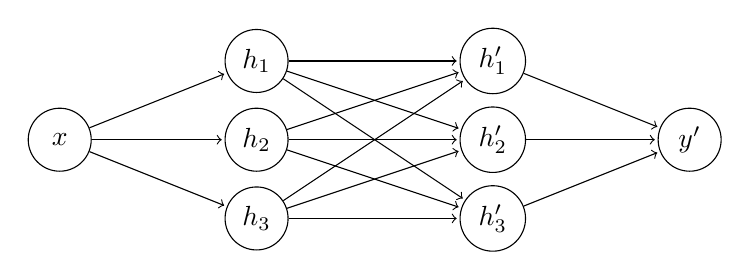
\begin{tikzpicture}[->, shorten >=1pt, auto, node distance=1.5cm, main node/.style={circle, draw, minimum size=0.8cm}]

        \node[main node] (x) {$x$};
        \node[main node] (h1) [right of=x, xshift=1cm, yshift=1cm] {$h_1$};
        \node[main node] (h2) [right of=x, xshift=1cm] {$h_2$};
        \node[main node] (h3) [right of=x, xshift=1cm, yshift=-1cm] {$h_3$};

        \node[main node] (h1') [right of=h1, xshift=1.5cm] {$h_1'$};
        \node[main node] (h2') [right of=h2, xshift=1.5cm] {$h_2'$};
        \node[main node] (h3') [right of=h3, xshift=1.5cm] {$h_3'$};

        \node[main node] (y) [right of=h2', xshift=1cm] {$y'$};

        \foreach \i in {1, 2, 3} {
            \draw (x) -- (h\i);
            \draw (h\i) -- (h1');
            \draw (h\i) -- (h2');
            \draw (h\i) -- (h3');
        }

        \foreach \i in {1, 2, 3} {
            \draw (h\i') -- (y);
        }
    \end{tikzpicture}
\caption{Visualization of a neural network with scalar input and output, and two fully connected layers, redrawn after Prince~\cite{princebook}.}
\label{image:neuralnet}
\end{figure}

The computation of an output based on an input in the network is called the 
feed-forward, as the computation runs layer by layer through the 
network. The process starts from the input layer, the input 
organized as a vector. Each intermediate value on a hidden layer, noted $h_d$ below,
is computed by taking a linear combination of the layer weight vector $\mathbf{\theta}$ and 
the input vector $\mathbf{x}$ of size $N$, adding the 
bias term $\theta_0$, and passing the result through the activation function $a$:

\begin{align}
    h_d = a\left[ \theta_{0} + \sum_{i=1}^{N}\theta_{di}x_{i} \right]
\label{eq:fc_layer}
\end{align}

Different types of layers, such as convolutional or transformer layers 
denote that this single-layer computation process is performed differently from 
the standard form. When many layer types are present, layers using the computation
in Equation~\ref{eq:fc_layer} are called fully connected or dense layers. The full computation of 
the feed-forward consists of performing this computation on each layer, finally producing the 
network output after up to hundreds of layers.

The universal function approximator theorem states that functions belonging to the 
neural network family are capable of approximating any mapping from any type or shape of input
to any output with arbitrary precision~\cite{princebook}. Naturally, due to high computational 
costs of finding the optimal weights,
this theoretical optimum is rarely reached.

Examples of input-to-output mappings that can be approximated with a neural network to solve a character recognition task are the following. The problem of character classification takes in an input image of a character and outputs which character is found on the image. The output is a probability vector, where each value notes the probability that the image contains the character this value is chosen to represent. The softmax activation function, found in Equation~\ref{eq:softmax}, is used before the output layer to force the output to contain valid probability values that sum to one. Generalizing the mapping problem further, one can also use as input an image 
with a text sequence, and teach a neural network to output the text on the image.
Due to the variable output length, a technique called sequence-to-sequence learning 
is employed~\cite{sutskever2014sequence}. This encodes the fixed-length output layer to variable-length 
output text. Even though the main problem of this work is to recognize characters, 
generally the term optical character recognition is used for detecting longer text sequences.

\begin{align}
    \text{softmax}_k[\mathbf{z}] = \frac{\exp[z_k]}{\sum_{k'=1}^{K} \exp[z_{k'}]},
    \label{eq:softmax}
\end{align}

Finding the best network weights for any of these types of input-to-output mapping problems, training 
a network, is conducted with the same process.
The general recipe for training a neural network is the subject of the next section.

\section{Training neural networks}
\label{sect:training}

After one has defined a neural network structure, initialized the weights of the network 
to some initial values, and obtained a sufficiently large set of input-output pairs from the problem at hand,
one can start training the network. Training is an iterative process where inputs are used to 
predict the output that is then compared to the ground truth. A more detailed account of these iterations
is presented next.

At the start of training, a small fraction, commonly 10-20\%, is reserved as test data. The remainder, 
the training set, is divided into small chunks called batches.
In an iteration of neural network training, a batch, stacked in a tensor of dimension one larger than the dataset, 
is passed through the network: outputs are computed based on the training inputs with the feed-forward process.
After this, a loss function is used to evaluate the quality of the output: the loss function maps the network output and 
the correct output recorded in the training batch and outputs a scalar value, a small value denoting a good 
match. Loss functions used in optical character recognition are presented in Section~\ref{sect:loss_funcs}.
After this follows a step called backpropagation: the gradient of the loss function with respect 
to the neural network weights is computed. The algorithm used in this computation is called automatic differentiation
and is able to compute gradients with equal computational complexity as the feed-forward by utilizing 
a variant of the chain rule and by proceeding backward in the network~\cite{princebook}.

Once the gradient is computed, the next step is to choose how to adjust the network weights 
based on the gradient information. The simplest approach is, given a predefined step size 
known as the learning rate, to adjust the weights by the magnitude of the learning rate 
in the direction of the fastest decreasing gradient, a heuristic called gradient descent. Different options for this approach 
are generally called optimizers and finding a suitable one is a fairly complex problem.
Other optimizers are stochastic gradient descent (SGD) that inserts randomness 
to the weight-adjusting steps, and Adam (Adaptive Moment Estimation) that 
uses moments or gradients obtained in previous steps to add smoothness to the 
movement trajectory~\cite{princebook}. After a weight-adjusting step is completed 
with the optimizer, the training iteration is completed.

The training process consists of repeatedly performing the aforementioned training 
iterations. Once all batches of the whole dataset are used for training,
a training step known as an epoch is completed, with common training processes 
completing dozens or hundreds of epochs. The training is terminated once a predefined 
stopping condition, such as a number of epochs or a sufficiently small gradient 
magnitude, is met. The goal of the training process is to find the global minimum of the loss 
function with respect to the network weights, as this setting would correspond to 
the optimal approximation of the input-output mapping. Like with optimizers, 
determining optimal stopping conditions is a difficult problem area within neural network optimization.

After the training is completed, the test dataset laid to the side at the start of 
training is used to evaluate the predictive power of the network on unseen data.
At this point, the model should be considered frozen, as adjusting it would 
optimize the model to the small test set, not the general problem. This pitfall is 
known as \textit{data leakage}~\cite{engbook}.

As is evident from the generality of the previous description, there are numerous 
aspects to consider when designing accurate neural networks. The 
rest of this chapter presents a snapshot of this problem area, focusing on those 
relevant to our problem of recognizing handwritten characters, and the rest of the 
work experiments with parts of these aspects. A summarizing pseudocode of the 
neural network training process with gradient descent is presented in Algorithm~\ref{alg:net_training}.

\begin{algorithm}
    \caption{Neural Network Training}
    \begin{algorithmic}[1]
        \State \textbf{Input:} training\_data, epochs, learning\_rate
        \State Initialize weights $W$
        \State Initialize biases $b$
        
        \For{epoch = 1 to epochs}
            \For{each (input, target) in training\_data}
                \State $output \gets \text{FeedForward}(input, W, b)$
                \State $loss \gets \text{CalculateLoss}(output, target)$
                \State $(gradients\_W, gradients\_b) \gets \text{BackPropagation}(input, output, target, W, b)$
                \State $W \gets W - learning\_rate \times gradients\_W$
                \State $b \gets b - learning\_rate \times gradients\_b$
            \EndFor
        \EndFor
        
        \State \textbf{Output:} $W, b$  \Comment{Trained weights and biases}
    \end{algorithmic}
    \label{alg:net_training}
\end{algorithm}

\subsection{Loss functions}
\label{sect:loss_funcs}

Loss functions are needed within the neural network training process to evaluate the model output 
quality in each training iteration. These functions map two equally shaped inputs, the predicted 
and true labels, to a scalar value describing match quality, a low value representing a good match~\cite{princebook}. 
For instance, the simple function $f: x,y \rightarrow |x-y|$  would qualify as a loss function.
The most commonly used loss functions in character classification for optical character recognition is 
the cross-entropy loss.

Loss functions are constructed using maximum likelihood estimation. When one frames the neural network as outputting 
a conditional distribution $P(y|X)$, $y$ being the network output, and $X$ the input, each correct label in the 
training set should have a high probability in this distribution. The likelihood is obtained by taking the product of 
all ground truth label occurrence probabilities, and the training goal becomes maximizing this value. Loss functions are derived 
from the maximum likelihood formalization so that the network parametrization associated with zero loss is equivalent to 
the maximum likelihood parametrization. These derivations are out of the scope of this work but can be found in Prince's book
Section 5.7~\cite{princebook} for the cross-entropy loss function.

The cross-entropy loss function maps pairs of class probability vectors 
to a loss value. The model output vector describes the probabilities 
of the input belonging to each of the possible classes, while the ground
 truth vector has the correct 
class set to one, and all other probabilities to zero. The loss function $L$ 
is constructed using the Kullback-Leibler divergence between the empirical data distribution $q(y)$,
a point mass distribution of the correct labels,
 and the model output distribution 
$Pr(y|\mathbf{\theta})$:

\begin{align}
    L(\mathbf{\theta})=\int_{-\infty}^{\infty}q(y)\log[q(y)]dy-\int_{-\infty}^{\infty}q(y)\log[Pr(y|\mathbf{\theta})]dy,
\end{align}

where the first term is omitted since it has no dependence on the parameters $\mathbf{\theta}$.
As the distributions are discrete, the loss reduces to

\begin{align}
    L(\mathbf{\theta})=-\sum_{i=1}^{N}\log[Pr(y_i|f(x_i,\mathbf{\theta}))],
\end{align}

where $N$ denotes dataset size, $y_i$ the correct label, and $f(x_i, \mathbf{\theta})$ is the neural network output. This is computed as the negative sum over all logarithms of the probability of the input being of the correct class according to the model. As all correct label probabilities are one, the perfect solution sets all logarithms to zero, making the loss value zero equivalent to the maximum likelihood solution.

Before training a neural network can be started, the network structure needs to be decided. The alternatives are called \textit{architectures}, most relevant of which for character recognition are presented next.

\section{Architectures}

Neural network architectures are alternative ways of constructing the network structure for cases where the standard variant presented in Equation~\ref{eq:fc_layer} is not ideal. Alternative layer types are used to make the model pay more attention to desired 
aspects~\cite{alexnet}, such as image structures ignoring their position in image processing, or features most usable for summarizing data in autoencoders.

This section presents layer types used in handwritten character classification 
along with model architectures that first introduced them.
These are convolutional layers, residual connections, autoencoders, and the multi-head self-attention operation used in transformer architectures, and are presented next.

\subsection{Convolutional layers}

The primary motivation for the introduction of convolutional layers was to find a way to encode general prior information 
on images to the network architecture: force the network, by adjusting its computational 
algorithm, to pay attention to particular aspects while ignoring others. Constraining the problem with priors allows reducing parameter count per layer, which frees up 
computational resources to training further and with more data~\cite{alexnet}.

The two pieces of prior knowledge encoded to the convolutional layer computation
 are invariance to geometric and pointwise transformations, and local relatedness of pixels~\cite{princebook}.
Transformation invariance states that morphing an image keeps its meaning: for instance,
 moving a letter A in an image, 
rotating it, coloring it red, or squishing it still preserves the fact of it being a letter A. Local relatedness 
encodes that most pixels next to each other have similar intensity values and that pixels cannot be shuffled without losing meaning. A visualization of these assumptions can be found in Figure~\ref{fig:conv_assumptions}.

\begin{figure}[ht]
    \centering
    \resizebox{0.7\linewidth}{!}{
        \begin{minipage}[b]{0.45\linewidth}
            \centering
            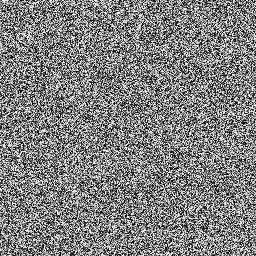
\includegraphics[width=\textwidth]{images/snowfall.png}
            \subcaption{An image with no nearby pixel similarity, such as this image made up of random numbers, is assumed to never occur among real-world images.}
            \label{fig:snowfall}
        \end{minipage}
        \hspace{0.4cm}
        \begin{minipage}[b]{0.45\linewidth}
            \centering
            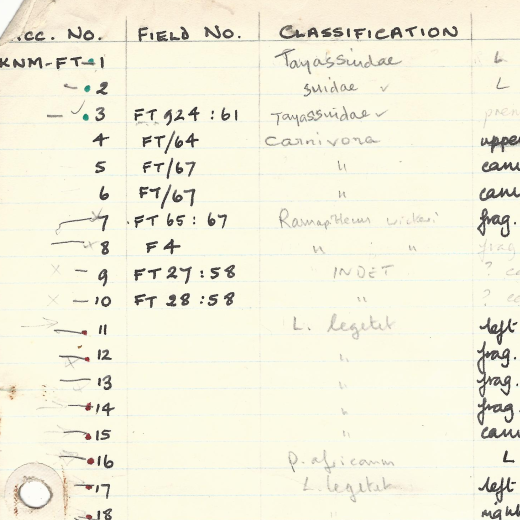
\includegraphics[width=\textwidth]{images/cataloguesample.png}
            \subcaption{In a real image, most pixel colors are almost equal to neighboring pixels. Segment from 
            the Fort Tenan Catalogue of the National Museums of Kenya.}
            \label{fig:snowfall2}
        \end{minipage}
    }

        \vspace{0.4cm}

    \resizebox{0.7\linewidth}{!}{
        \begin{minipage}[b]{0.45\linewidth}
            \centering
            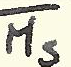
\includegraphics[width=\textwidth]{images/molar.png}
            \subcaption{Transform invariance: the original tooth notation sample...}
            \label{fig:snowfall3}
        \end{minipage}
        \hspace{0.4cm}
        \begin{minipage}[b]{0.45\linewidth}
            \centering
            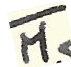
\includegraphics[width=\textwidth]{images/rotated_molar.png}
            \subcaption{... still keeps its meaning of lower third molar after a transform}
            \label{fig:snowfall4}
        \end{minipage}
    }

    \caption{Visualization of the similarity and transform invariance assumptions encoded in the convolutional layer computation.}
    \label{fig:conv_assumptions}
\end{figure}

The layer output computation on a convolutional layer is similar to the fully connected layer computation
presented in Equation~\ref{eq:fc_layer}, but takes as input only a small region around each pixel and uses the same weight parameters on all input positions. To achieve this, the layer weights form a small matrix called kernel~\cite{princebook}. During the computation, the kernel 
acts as a sliding window, producing the output for each position by computing the dot product between the kernel and the kernel-sized input region around the processed position, and as usual, a bias term is added and the result passed through a nonlinear activation function. An illustration of convolution in the color image case, where the kernel is three-dimensional,
is found in Figure~\ref{image:3dkernel}.

\begin{figure}[ht]
    \centering
    \includegraphics*[scale=0.4]{images/3dkernel.png}
    \caption{An illustration of a convolution computation in the case of a color image, from Prince~\cite{princebook}.}
    \label{image:3dkernel}
\end{figure}

Usually, a convolutional layer is followed by a pooling layer~\cite{princebook}. The pooling layer adds more nonlinearity to the network and allows reducing layer sizes. The most common operation is the max pooling operation, where each output pixel is the maximum of
a 2x2 area in the input. Other, less popular operations include using mean or average in the pooling operation. These operations allow for the common structure of convolutional networks, where the layer output size progressively decreases as the computation proceeds.

Many advances in convolutional networks have been motivated by the ImageNet image classification competition~\cite{imagenet}
 that ranks models by their capacity of classifying images retrieved from the web to 1\,000 distinct classes.
 The results are presented as top-1 and top-5 error rates, the percentage of samples 
where the correct class is not among the one or five most likely classes according to the network. As convolutional architectures
that have performed well in the competition have been found valuable in handwritten character classification, the 
breakthrough models presented next are experimented with in later parts of this work.
These most influential convolutional models in the history of the ImageNet challenge  that
only rely on the basic convolution operation, are AlexNet~\cite{alexnet}, 
the VGG model family~\cite{vgg}, and
the Inception architecture used in GoogLeNet~\cite{googlelenet}.

The AlexNet convolutional neural network is perhaps the most influential deep learning model of all time, 
popularizing deep learning as a superior feature extractor compared to human-performed feature engineering~\cite{princebook}.
The breakthrough was mainly achieved by speeding up the training process with graphical processing units, a novel idea at the time, and simplifying the feed-forward computation by replacing the
hyperbolic tangent activation popular at the time with the ReLU function~\cite{alexnet}.
 This allowed training a larger, deeper network
with convolutional kernels up to the size of 11x11, leading to nearly halving the best top-5 error rate with the score of
17.0\%. Other, more minor but still highly influential innovations were the normalization of convolution results, 
overlap in pooling areas, and dropout regularization, a heuristic where connections are randomly dropped to avoid over-reliance on certain connections~\cite{dropout}.

The ImageNet competition of 2014 saw the next breakthrough innovation with the winning architecture GoogLeNet~\cite{googlelenet}. The authors
introduced smaller convolutional kernels with highly optimized training computation that allow deeper,
and therefore more capable networks. The layer architecture, named Inception after the ``We 
need to go deeper'' internet meme~\cite{we_need_to_go_deeper}, only used kernels of size 3x3 and 5x5, and
employed layer channel count reduction with 1x1 convolutional kernels. Sparsity by omitting connections was introduced on dense layers, inspired by knowledge of the structure of biological visual systems. While these ideas were motivated
by performance-related reasons, to reach as high accuracy as possible with a fixed count multiple-add operations in training, the resulting model ended up reaching a new best top-5 error rate of 6.75\%
in ImageNet classification.

A close runner-up in the 2014 competition, the VGG model family again proved that deep networks 
with small kernels outperform shallow, larger-kernel approaches~\cite{vgg}. The experiments included fixing all kernels to 3x3 size, and benchmarking classification accuracy between 
different model depths. The deepest model with 19 layers was found to be the most accurate, and highly competitive as a feature extractor: an appendix of experiments reached new-best results on a variety of 
further classification tasks. While the 
best top-5 accuracy of 7.3\% ended up with second place in the ImageNet 2014 competition, the structural simplicity
and diverse learning capacity of the VGG models had a major influence on later deep learning research.

The architectures of the AlexNet, GoogLeNet, and VGG models are summarized in Figure~\ref{image:famouscnns}.

\begin{figure}[ht]
    \centering
    \includegraphics*[scale=0.6]{images/famouscnns.png}
    \caption{Architectures of AlexNet~\cite{alexnet}, GoogLeNet~\cite{googlelenet}, and VGG-16~\cite{vgg}, the 
    VGG model variant with 16 layers, from Zhang~\cite{zhangImagebasedMethodsDietary2023}.}
    \label{image:famouscnns}
\end{figure}

\subsection{Residual connections}

Following the success of increasingly deep networks~\cite{vgg,googlelenet}, the question arose of whether 
achieving better approximation capacity with a neural network solely was about stacking more layers~\cite{resnet}.
The previous major problem of vanishing and exploding gradients had been solved by input and between-layer 
normalization operations. The vanishing gradient problem refers to when the gradient of the loss with respect to 
some parameters becomes zero, these parameters can no longer be updated by adding any learning rate multiplied by the gradient. Exploding 
gradients lead to numerical instability as the optimum is best approached gradually rather than adding very large numbers to weights. Normalization solves these problems by updating activations to a consistent distribution, avoiding gradients getting stuck to extreme values~\cite{batchnorm}.
However, after stacking even more layers with the help of normalization operations, another issue, the degradation 
problem occurred. This refers to the phenomenon where when iteratively training deeper networks, the accuracy 
reaches a peak and then starts degrading~\cite{resnet}. This suggested that there was something dysfunctional in 
the conventional deep network computations that started showing symptoms when a sufficiently deep network was trained.

As a solution to the degradation problem, He et al.~\cite{resnet} presented residual connections.
The premise was that if you add a skip connection that can bypass any layer computation, 
the deeper network contains in itself all the shallower variants and the resulting accuracy can never 
be worse than in a shallower network. The skip connection was implemented by adding the input to the layer output, the full computation becoming
$F(x) + x$ when expressing the layer without skip connection as $F(x)$.
Empirical results showed that this solved the degradation issue, and led to a 
vast improvement in classification accuracy. It was hypothesized that the reason for the degradation problem 
was that the deeper the network, the harder it is for the highly nonlinear network to approximate identity mappings, and when 
the depth passes a certain threshold, this drawback outweighs the added benefit of more layers. As the skip 
connection makes approximating the identity mapping very easy by setting all parameters but the skip connection to zero, the problem is eliminated. The results were impressive: 
The ResNet architecture won multiple image detection and segmentation competitions, including the ImageNet challenge 
of 2015, where the new best top-5 error of 3.57\% was reached with a network eight times deeper than the deepest VGG architecture~\cite{resnet}.

\subsection{Autoencoders}
\label{sect:autoencoders}

As one of the main ways to improve neural network accuracies is to obtain larger labeled datasets, various methods have been developed to increase dataset sizes without adding more manual labeling effort. As the best way to increase dataset 
size without adding labeling effort is to not use labels at all, self-supervised deep learning has been proposed 
as a solution~\cite{goodfellow}. In self-supervised learning, the correct output of the network is
derived from the input with a deterministic algorithm. This output is called a \textit{latent variable}.
Latent variables can be obtained, for example for images by hiding part of the image given to the network
and using the whole input as the output, or by adding noise to the input~\cite{princebook}.
The learning setting is constrained so that learning the latent variable 
based on the input remains a nontrivial task for the model.

Autoencoders are neural networks trained in a self-supervised manner to learn the identity function: the latent 
variable is the input~\cite{goodfellow}. To avoid situations where the network could trivially copy the values from 
the input layer to the output, the network is constrained. The most common way for this is to implement an undercomplete
autoencoder that has hidden layer sizes smaller than the input, forcing the network to find a way to distill 
the input data in a way that keeps as much of the original as possible recoverable on the output layer.
Another way of constraining the model is to add regularization parameters to the 
loss function, encouraging, for instance, small-valued or sparse parameters, rather than the trivial solution.

The natural follow-up question to ask on autoencoders is why bother; what the utility 
of learning identity functions is. For the undercomplete autoencoder, the computation 
can be interpreted as a mapping from the input to a compressed representation $h$, and 
another computation from $h$ to the input; an autoencoder is a function $x\to h\to x$~\cite{goodfellow}.
The utility lies in this hidden unit $h$ and that one can take out only the 
computation from $x$ to $h$, called the \textit{encoder}, or from $h$ to $x$, the \textit{decoder}.
From the perspective of image classification, the encoder is most useful as it serves 
as a powerful feature extractor: one approach for creating a character-recognizing model 
is to first train an autoencoder and then train a classifier by appending 
fully connected layers to the encoder, an approach successfully implemented for the Bangla language~\cite{6shoponBangla}.
Thus, autoencoders can be used as the source 
task in transfer learning, as discussed in Section~\ref{sect:transfer_learning}.

\subsection{Transformers and the multi-head self-attention}

The multi-head self-attention layer present in transformer architectures was
originally motivated by natural language processing tasks, as other layer types
encode prior knowledge of language poorly.
Convolutional layers can only use the immediate neighborhood of the input for activation computations, making it impossible to attend to other words far in a sequence, which would be necessary for text processing. Fully connected layers would cause parameter counts to become insurmountable large as input sizes for language models are huge: sequences are processed by splitting the sequence into tokens, such as words, and generating \textit{embeddings}, long numeric vectors describing tokens and their positions~\cite{princebook}.

To construct the self-attention operation, the nature of language was studied 
as an information retrieval problem: a primitive search engine is used as an analogue to construct a way to rank content by relevance.
The \textit{query}, a string of characters, is used to rank \textit{keys}, web pages. This is done by computing a similarity metric: checking how many words in the query appear on each web page. The
the result is a list of \textit{values}, web pages ordered by their relevance ranking.

The process for constructing the output for each input token embedding follows a similar process.
For the input, one embedding vector, the similarity to all other token embeddings is computed with cosine similarity, given in Equation~\ref{eq:cos-similarity}. This similarity metric computes the cosine of the angle between two vectors using the dot product and scales it by vector magnitudes,
 giving a scalar metric with one denoting perfect similarity and -1 perfect dissimilarity. As the similarity is also computed between the input and itself, this \textit{attention} value becomes 1.
The name \textit{self-attention} stems from this phenomenon of parts of a sequence attending to themselves. Finally, the \textit{attention} value obtained for each embedding pair is combined to a representation of a relevance-ranked list by multiplying the attention by the token embedding creating output values with larger values representing how much attention should be paid between each pair.

\begin{align}
    \text{Cosine similarity}(\mathbf{k}, \mathbf{q}) = \frac{\mathbf{k} \cdot \mathbf{q}}{\|\mathbf{k}\| \|\mathbf{q}\|}
    \label{eq:cos-similarity}
\end{align}

A few technical adjustments to the aforementioned process are made for the self-attention layer to summarize notation and add learnable parameters. To represent the whole computation with one equation, all token vectors are collected in the input matrix $X$. Three copies of this matrix are created for the queries, matrix $Q$, keys, $K$, and values, $V$, by introducing learnable parameter matrices $W_K, W_Q$, and $W_V$, and multiplying the input matrix $X$ by each. The similarity values are computed by multiplying the query and key matrices and dividing the result by the square root of the token length. The denominator differs from cosine similarity, but this avoids the need to compute vector norms and preserves the ordering between attention values. The attention matrix is obtained by passing the similarities through the softmax function (Equation~\ref{eq:softmax}) to scale them to values between zero and one. Finally, the relevance-ordering representation is constructed by multiplying the attention matrix with the value matrix $V$. This forms the dot-product self-attention computation, summarized in Equation~\ref{eq:self-attention}.

\begin{align}
    \text{Self-attention}(\mathbf{X}) &= \text{softmax} \left[ \frac{\mathbf{Q}\mathbf{K}^T }{\sqrt{d_k}} \right] \mathbf{V}, \label{eq:self-attention} \\
    \nonumber\text{where} \quad \mathbf{V} &= \mathbf{X} \mathbf{W}_v, \; \mathbf{K} = \mathbf{X} \mathbf{W}_k \; \text{and} \; \mathbf{Q} = \mathbf{X} \mathbf{W}_q.
\end{align}

With the self-attention operation, one limitation remains: one attention layer is only able to focus on one aspect of the 
input sequence at a time. To allow multiple interpretations, in \textit{multi-head self-attention}, many self-attention operations are run in parallel. To preserve the weight matrix sizes, each token embedding is split across the heads and the 
results from the value matrix multiplied with the attention matrix are concatenated back together. The self-attention operation with multiple heads is summarized in Figure~\ref{fig:multi-head-self-attention}.

\begin{figure}[ht]
    \centering
    \includegraphics*[scale=0.57]{images/multiheadattention.png}
    \caption{Multi-head self-attention with two heads, from Prince~\cite{princebook}.}
    \label{fig:multi-head-self-attention}
\end{figure}

The main premise of the transformer architecture is that the multi-head self-attention 
is the only operation required to successfully learn nature language processing tasks~\cite{attention_is_all_you_need}. The first transformer model,
an autoencoder only using transformer blocks with a multi-head self-attention and 
a fully connected layer both followed by batch normalization and with a residual connection, achieved a new best 
result in machine translation from English to German by a significant margin~\cite{attention_is_all_you_need}.
The most famous application of attention-based models is, however, a model taught to continue a sentence fragment with the next most 
likely character. The chat-style variants of these models, the most famous being ChatGPT by OpenAI, have become well-known among the general public and 
have been speculated to show signs of general artificial intelligence.

In computer vision, transformer architectures have been successfully implemented.
The most notable of these is the Vision Transformer (ViT)~\cite{vit} that achieved a top-1 error rate of
11.45\% on the ImageNet challenge, an impressive result yet less accurate than the best convolutional networks of the time.
Falling behind convolutional networks was likely due to lacking prior knowledge of images encoded in the convolution operation, nearby pixel similarity, and
translation invariance, leading to larger requirements of data and computational resources 
to reach high accuracies. Still, transformer architectures are actively experimented with in many computer vision tasks, including handwritten character classification~\cite{9thuonPalm}.

The layer computation variants presented in this section; convolution, residual connection, encoder-decoder chain, and 
the multi-head self-attention form the set of alternatives commonly used for image classification. Models built with these mechanisms 
have achieved impressive accuracies in classifying the ImageNet samples according to what can be seen in each image.
To utilize these models in handwritten character recognition, a mechanism for applying this knowledge to a new task is required.
This is called transfer learning and is presented next.

\section{Transfer learning}
\label{sect:transfer_learning}

Much of transfer learning is about what happens before training a neural network is started: using an architecture and starting training from a parametrization already successful at a related task
is known to result in a better model~\cite{transferlearning_survey}. As an analogue to human learning, teaching a human transcriber to read fossil specimen markings is easier if the person already knows how to read.

Transfer learning benefits constructing neural networks 
by aiding in optimization, generalization, and regularization, and saving computational resources and labeling effort~\cite{erhanWhyDoesUnsupervised2010, transferlearning_survey}.
Erhan et al.~\cite{erhanWhyDoesUnsupervised2010} found a theoretical explanation for these benefits: they
experimented with ordering the training data and found 
that early examples have a significant influence on the learning trajectory trapping the optimizer in a parameter region that is later hard, 
if not impossible, to escape. Therefore, seeing examples from another learning task prevents overfitting by preventing the optimizer from getting trapped in undesirable parameter regions. As the model also sees more versatile examples, it is known that the result generalizes better~\cite{transferlearning_survey}.
The practical implementation of transfer learning is better understood when one views a neural network as a hierarchical feature extractor:
The first layers learn low-level features of the input, and downstream layers combine these to higher-level concepts.
In the letter-recognition case, a low-level feature could be noticing edges, and a higher-level feature that the edges curve and intersect in 
specific ways. As lower-level features are common between tasks, they can be reused by fixing the first layers, also called \textit{freezing} layers,
and adjusting only the lower layer parameters during training.
Freezing parameters reduces the search space for optimal configuration of the remaining parameters, saving computational resources. Additionally, the required quantity of labeled training data is reduced, saving on one of the most laborious aspects of creating deep networks~\cite{engbook}.
A way to circumvent even more labeling is using a self-supervised learning task, such as an autoencoder, as discussed in \ref{sect:autoencoders}. Taking this a step further, source models trained in a self-supervised manner on huge data sets and being usable for almost any target task are called \textit{foundation models} and have gained significant research attention lately. However, even in cases where labeled training data is abundant, pretraining on another dataset is beneficial likely due to the generalization and early example influence aspects~\cite{erhanWhyDoesUnsupervised2010}.

While the principle of transfer learning was known by a variety of names before, the first survey on the topic~\cite{transferlearning_survey} collected all these ideas under the term transfer learning and established further terminology related to the paradigm. The first problem solved by the model is called the source;
the mapping $X\to y$ is termed the \textit{source task}, and the input and output pair distribution $P(y|X)$ is termed the \textit{source domain}.
Similarly, the next task solved is called the target, with mapping being the \textit{target task} and the data distribution the \textit{target domain}.
A less rigorously defined term for referring to the similarity of the source and the target is \textit{transfer distance}. Transfer learning is further divided into subcategories according to whether source and target tasks or domains differ. In our task, where the source is image classification and the target is character classification, tasks differ, which is a problem of \textit{inductive transfer}.
As both features and hyperparameters are re-used, both \textit{feature representation transfer} and \textit{parameter transfer} are implemented. Should one in the future want to fine-tune the models 
developed in this work with catalogues from another institution, only the domains would differ, creating a \textit{transductive transfer} setting with a much shorter transfer distance than in our case.

In the literature review and experiments, it is assumed that starting training from a random parameter initialization, \textit{from scratch}, in no case works 
better than transfer learning, a consensus largely shared among the machine learning community~\cite{cs231n_transfer_learning}.
For this reason, research works implementing new character set recognition by training from scratch are omitted from the literature search.

\bigskip
\noindent This chapter presented background on neural network training relevant to the task 
of classifying handwritten digits. The coarse principles to remember for the following chapters 
are that a neural network essentially is a function approximator. The different structures are 
used to aid in this approximation by encoding prior knowledge; the convolution operation encodes these 
for images, and the self-attention for text sequences. Autoencoders are used to conduct self-supervised
learning, where output equals the input. Neural network training refers to finding the best 
parameters to approximate the given mapping, and is conducted iteratively by creating 
an output, comparing it with the correct output, and adjusting the parameters in the direction 
of better output-producing parameters. Transfer learning means that this process is started with a 
 parametrization that is assumed to be closer to the best parametrization than an average 
random initialization. The following chapters review previous experiments implementing 
neural network training with transfer learning to solve the task of character image classification and experiment with previously successful approaches to correctly classify handwritten tooth fossil markings.

\chapter{Related Work}

This chapter presents related work from two viewpoints. First, in Section~\ref{sect:related_same_problem},
work on digitizing handwritten fossil catalogues is reviewed. As the work 
in this area is highly limited, Section~\ref{sect:same_solution} presents work using similar techniques 
to ones used here: publications aiming to recognize individual handwritten characters 
with deep neural networks and transfer learning with limited target domain data.

Literature to review was selected with a snowball search, proceeding with forward and backward citations 
of key articles. Additionally, the last five to ten years of conference proceedings most relevant for this problem area were 
scanned. For related work on fossil digitization, any found work touching on the subject area is commented on due to their 
limited amount. For work conducting a similar analysis of handwritten character recognition, more strict conditions were placed. 
For results, to be considered, the work had to be explicit about the best accuracy score achieved,
mentioning the size of the training dataset, the number of characters within the classification problem, and accuracy on the test set.
 The source of the base model had to be given along with its source task, training data, and network architecture. The exact method of conducting the model fine-tuning had to be explicit enough to be reproducible,
work only stating they used transfer learning or leaving gaps in the training process were omitted. Additionally, 
presentation quality was taken into account by omitting some work due to
 undecipherable or missing details.

\section{Approaches to digitization of handwritten fossil catalogues}
\label{sect:related_same_problem}

While digitizing handwritten fossil catalogues holds,
should all state-of-the-art optical character recognition and data management methods 
be in full use for solving the problem, perhaps a dramatic potential for improving 
the quality of paleoecological research, little has as of now been done in this area.
Likely due to the problem having attracted little attention, 
most current work assumes the most rudimentary method: a person sitting down, and transcribing.

Due to large amounts of transcription work already done, there are digital repositories of fossil data.
Uhen et al.~\cite{uhenCardCatalogsComputers2013} review such databases and encourage further 
digitization of unpublished data, but do not take a stand on how one should complete such work.
Another more extensive review, a whole chapter on digitization methods in paleontology has been written~\cite{mallisonDigitizingMethodsPaleontology2011},
but the chapter exclusively considers digitizing physical bone and plant pieces with various 3D imaging methods.

For automated handwriting recognition, a few mentions exist in previous work. The data management themed 
article by Groom et al.~\cite{groomImprovedStandardizationTranscribed2019} identifies the primary 
problem of this thesis: it is mentioned that most fossil data exists as handwritten records with sufficient information 
to conduct analysis without the physical sample, and that a big advancement in data availability would be to efficiently and 
systematically convert this data to a structured database. Optical character recognition is presented, but more as a futuristic option 
not feasible with current methods, and any data quality suggestions implicitly assume that transcription is completed 
by a human. This review is still relevant for automated digitization as many important considerations in data structuring,
standardization, and quality management are presented - revealing the new challenge that should large-scale automated digitization succeed,
the next big line of work would be how to structure and manage the digital paleontological data.

The only found work solving the exact same challenge as this work is the article by Shanmugavel et al.~\cite{shanmugavelHandwrittenOpticalCharacter2018}.
While the task is exactly the same, the methods only contain basic computer 
vision processes, edge and contour detection, and a lack of results reveals that not much was achieved in 
this project. However, it serves as proof that such attempts have taken place in previous years.

Concluding the review of research articles on digitizing handwritten fossil data, it seems that no successful projects
have as of now been completed outside of the Data Science student project in spring 2024 for the National 
Museums of Kenya, for which this work is a continuation. Therefore, the experiments in this thesis
start with the simplest problem reductions and only present more advanced techniques as ideas for future work.
The rationale behind this decision is that since not much has yet been done, it is best to start from 
simple and established implementations to verify simple hypotheses before proceeding to more recently developed methods.

\section{Approaches to handwritten character recognition with small target domain datasets}
\label{sect:same_solution}

Due to the limited amount of work on optical character recognition on fossil catalogues, other 
domains were chosen to draw inspiration from for constructing the model training setting. 
Interestingly, the nature of the fossil catalogue digitization problem has much in common with 
reading regional Sanskrit-based South Asian languages, and with certain historical 
scripts, due to the following similarities.
Firstly, the available data is small. While on first thought, languages where characters compound of
 multiple smaller units such as  Chinese or Korean would be more applicable, these are not
  generally solved with transfer learning as the datasets are sufficiently large to train from scratch.
Several of the South Asian languages contain modifiers \cite{2limbachiyaGujarati,3chatterjeeBengali,5rasheedHandwrittenUrduWAlexNet},
recognizing which can be seen as analogous to under- or overlines in the dental markings.
Many characters are cursive in nature~\cite{5rasheedHandwrittenUrduWAlexNet}, which makes
 especially character segmentation 
solutions more applicable as both the Asian languages and fossil catalogues face similar challenges.
The last trait that makes recognizing characters in these languages similar to dental markings is that character sizes vary~\cite{6shoponBangla},
which is also the case with the smaller upper and lower script characters in fossil catalogues.
For the historical scripts, a study on machine reading historical manuscripts written on palm leaves was 
included as the scanning of these scripts is more challenging due to the old leaves, and the 
study therefore contained valuable insight on image quality enhancement techniques~\cite{9thuonPalm}. Additionally, historical scripts 
contain far more characters than modern languages, making the problem more challenging and therefore more interesting.

To note on all articles reviewed in this section is that the analytical basis was incomplete: reasons for why a technique 
was chosen to be implemented over reasonable alternatives were largely missing, and transfer distance considerations were 
mostly omitted. This has a number of consequences. The reasoning behind method selection could not be evaluated. The rationale 
behind some decisions, such as flipping characters as a data augmentation technique~\cite{9thuonPalm}, optimizing the hyperparameter for character
 rotation angle in data augmentation~\cite{7rizkybasicCnnTransfer} or using data augmentation on the test set~\cite{11zunairUnconventionalWisdom}, could benefit from 
 further clarification. Not clearly defined metrics are used, such as positive-to-negative rates~\cite{10goelGujarati, 5rasheedHandwrittenUrduWAlexNet} that lack a definition for 
 the multi-class case and an explanation of the cost differences between the error types. For specifications, the lack of analytical
  basis results in missing necessary details, such as the implementation of layer freezing~\cite{8goelGujarati2023}, and the inclusion of redundant information,
   such as hardware specifications when runs are not timed~\cite{9thuonPalm}. Even the goal of the study was occasionally not as well motivated: one 
   study justified compromised result accuracy by training for fewer epochs~\cite{3chatterjeeBengali}, even though training with transfer learning can typically 
   be completed in order of minutes, even on a CPU. For these reasons, some unexplored alternatives are used in this
    thesis as previous work cannot invalidate their viability.

While not directly analogous, a few works acted as major inspirations on aspects of the solution implemented in this work.
Zhao et al.~\cite{4zhaoTibetan} achieved new state-of-the-art accuracy in multi-style Tibetan glyph classification
with a model chain approach that first classifies glyphs by style and then recognizes the glyph with a style-specific model. As these downstream
 residual learning models are trained with transfer learning with a Tibetan 
 recognition base model, the similarity of source and target data domains makes the transfer setting more simple than with
the fossil catalogues. However, the approach of 
  chaining simple classifiers as a solution to a more complex problem served as an inspiration for
   the pipeline approach implemented in this thesis.

As another pipeline approach for detecting characters out of a longer sequence, Akhlaghi et al.~\cite{1akhlaghiFarsi} implemented 
a reading system for Farsi phone catalogues by chaining a gradient histogram-based segmentation 
algorithm with a digit classifier. While the segmentation task is due to uniform character
 sizes much simpler than the catalogue case, the work has a useful literature review on
  character segmentation. For classification, a small convolutional network was trained
   from scratch to a satisfactory accuracy of 94.6\%, proving that with careful architecture design,
    even small models can learn to accurately classify digits.

The rest of the literature reviewed in this section is directly analogous 
to the fossil case: an ImageNet or autoencoder base model is trained with transfer learning to detect a new set of characters.

Rasheed et al.~\cite{5rasheedHandwrittenUrduWAlexNet} created an AlexNet-based Urdu recognition 
model, achieving 98.12\% accuracy in digit recognition. The common last-layer replacement 
with a fully connected layer with softmax activation was benchmarked against using AlexNet as 
a feature extractor before support vector 
machine classification, the former giving the best result.

For Bangla character classification, Chatterjee et al. reported 96.12\% accuracy 
by fine-tuning a ResNet model. The work employed highly sophisticated transfer
 learning and learning rate scheduling algorithms, aiming to converge training in as 
 few epochs as possible, an aspect already discussed not to be as significant as a high test accuracy.
  Another concern was the concluding statement, ``if those misclassified points were 
  removed from the dataset, the accuracy will improve further'', which raises questions about the experimentation practices.

In Bangla digit classification, Shopon et al.~\cite{6shoponBangla} implemented self-supervised 
pretraining and found a new best accuracy in Bangla digits,
and the best accuracy among all articles reviewed, of 99.5\% by chaining an autoencoder
with a deep convolutional network. This proves that while less popular, approaches based on self-supervised pretraining are worth experimenting with.

Lastly for the Bangla language, Zunair et al.~\cite{11zunairUnconventionalWisdom} experimented 
with unconventional transfer learning approaches to classify digits.
The authors experiment with freezing layers below not frozen layers, a counterintuitive 
technique as later layer computation is dependent on the output of the previous ones.
Another unconventional approach involved immediately freezing the last fully connected layer, 
hindering any updates to the randomly initialized weights. The result of 97.09\% is stated 
to prove that these unusual approaches are worth experimenting with further, but due to this 
result being only found with one data set and one base model, and in the absence of solid 
theoretical basis, more evidence is required to justify the effectiveness of this method.

Several articles detected characters from the Gujarati language.
Goel et al.~\cite{10goelGujarati} were the first to attempt deep learning for Gujarati digits, 
achieving 96.5\% accuracy with the EfficientNet architecture. However, the authors utilized 
validation error on the test set as a stopping condition and then reported accuracies 
on the same set, leading to data leakage and a result not necessarily representative of true
generalization capability. In a later article~\cite{8goelGujarati2023}, the authors expanded 
their experimentation to other architectures, created several transfer learning settings informed 
by analysis on source and target task similarity, fixed the data leakage issue, and reported an 
improved accuracy of 97.92\%, again with the EfficientNet architecture. Additionally, adding a fully
connected layer is found to outperform using a support vector machine as the downstream classifier.
Limbachiya et al.~\cite{2limbachiyaGujarati} implemented digits and letters detection by comparing various convolutional architectures,
 achieving the best accuracy of 97.03\% with the MobileNet architecture. Transfer learning was implemented with a
  less usual top layer architecture: dropout was added between the two new fully connected layers.

As the only work reading characters from a benchmark dataset of handwriting, Rizky et al.~\cite{7rizkybasicCnnTransfer}
first compared various architectures and then used the best model, VGG16, to compare multiple transfer learning 
approaches. The final accuracy of 98.16\% was reached by fine-tuning the whole network. However, to achieve this accuracy, the exact best data augmentation parameters of 
rotation angle, image scale, and blur style are searched for, raising concerns about the real-world generalizability of this result.
 While the dataset is likely to be easier than fossil catalogues, the relative accuracy of
various approaches can give valuable insight to inform choices in designing the dental marking recognition system.

Lastly, an interesting application domain of reading characters used in ancient historical scripts written 
on palm leaves, Thuon et al.~\cite{9thuonPalm} achieved an impressive accuracy of 93,55\% on more than 100 
classes from challenging palm leaf scan images. The work includes many valuable parts: image enhancement,
data augmentation, and dataset expansion ideas, and comparison of multiple convolutional and attention-based 
architectures. As the main result, it is concluded that convolutional networks tend to outperform transformer architectures.

Details on all the works presented above are summarized in Tables~\ref{tab:dataset-info} and~\ref{tab:model-info}. Where multiple settings 
were experimented with, the class count producing the highest accuracy score and the three best 
base model variants are listed for brevity. The Tibetan detection article~\cite{4zhaoTibetan}
is omitted due to the transfer setting being different from the other works. Replacing the last layer with a 
softmax layer with an output size equal to the target class count is not 
stated in the table as it is done in every case. The shorthand 'FC' is used to denote a fully connected layer.

\begin{table}[h!]
\centering
\resizebox{\textwidth}{!}{
\begin{tabular}{|c|l|c|c|}
\hline
\textbf{Article} & \textbf{Language} & \textbf{Number of Classes} & \textbf{Samples per Class} \\ \hline
\cite{1akhlaghiFarsi}                & Farsi             & 10                         & 8,800                       \\
\cite{2limbachiyaGujarati}                & Gujarati          & 54                         & 1,400                       \\ 
\cite{3chatterjeeBengali}                & Bangla            & 84                         & 1,977                       \\ 
\cite{5rasheedHandwrittenUrduWAlexNet}                & Urdu              & 10                         & 840                        \\ 
\cite{6shoponBangla}                & Bangla            & 10                         & 2,922                       \\ 
\cite{7rizkybasicCnnTransfer}                & English           & 36                         & 2,055                       \\ 
\cite{8goelGujarati2023}                & Gujarati          & 10                         & 800                        \\
\cite{9thuonPalm}                & Ancient Balinese (1), Sundanese (2), Khmer (3) & 100 (1), 111 (2), 60 (3) & 193 (1), 1,836 (2), 122 (3) \\
\cite{10goelGujarati}               & Gujarati          & 10                         & 250                        \\
\cite{11zunairUnconventionalWisdom}               & Bangla            & 10                         & ~8,500                     \\ \hline
\end{tabular}
}
\caption{Literature Summary: Datasets}
\label{tab:dataset-info}
\end{table}


\begin{table}[h!]
\centering
\resizebox{\textwidth}{!}{
\begin{tabular}{|c|c|l|l|}
\hline
\textbf{Article} & \textbf{Best Accuracy} & \textbf{Base Model(s)} & \textbf{Transfer Method} \\ \hline
\cite{1akhlaghiFarsi}                & 99.37\%                & New Architecture       & -                        \\
\cite{2limbachiyaGujarati}                & 97.03\%                & MobileNet, DenseNet, VGG16 & Train new FC layer + dropout + output \\
\cite{3chatterjeeBengali}                & 96.12\%                & ResNet50               & Train all layers, increase learning rate for later layers \\
\cite{5rasheedHandwrittenUrduWAlexNet}                & 98.21\%                & AlexNet                & Train all layers but last layer most \\
\cite{6shoponBangla}                & 99.5\%                 & Autoencoder (trained on Bangla) & Append small deep CNN to autoencoder, no freezing \\
\cite{7rizkybasicCnnTransfer}                & 98.16\%                & VGG16, DenseNet121, ResNet18 & Train all layers        \\
\cite{8goelGujarati2023}                & 97.92\%                & EfficientNetV2S, Xception, ResNet101                    & Train all fully connected layers \\
\cite{9thuonPalm}                & 91.85\%                & EfficientNetB0, EfficientNetB1, ResNet101 & Freeze first layers \\
\cite{10goelGujarati}               & 96.5\%                 & EfficientNetV2S, InceptionV3, ResNet101 & Add 2 FC layers + output layer, no freezing \\
\cite{11zunairUnconventionalWisdom}               & 97.09\%                & VGG16                  & Freeze layers 16-20 (3 convolutional, 1 pooling layer) \\ \hline
\end{tabular}
}
\caption{Literature Summary: Accuracy, Base Model, and Transfer Method}
\label{tab:model-info}
\end{table}

This chapter presented work related to the problem of recognizing handwritten dental 
fossil markings. Since little work on fossil catalogues exists, the attention 
was turned to a related problem on an abstract level; recognizing handwritten letters
and digits in South Asian languages. The insight gained from the 
literature review is used in creating the training setup for the dental marking detection models.

\chapter{Experimental Setup}

The goal of this thesis is to recognize tooth type,
jaw, and index number markings to increase the accuracy of the element description in
the digitized fossil dataset of the National Museums of Kenya, ultimately aiming to improve the quality of paleoecological data analysis by improving the precision of the digitized catalogues. This 
chapter presents an end-to-end system that achieves this goal and gives reasoning 
for the training setups tested to build the required deep learning models.

The main hypothesis is that accurately recognizing tooth notation in catalogue images 
is best completed with a divide-and-conquer approach: by decomposing the main problem into small
subproblems of simple univariate classification, and chaining these to a tooth detection pipeline,
the subproblems become easy enough to be solved with perfect accuracy on limited data.
The experiments aim to verify the plausibility of this approach and find the most accurate deep 
learning models to solve the subproblems involved.

This chapter is organized as follows. In Section~\ref{sect:problem-formulation}, the tooth recognition problem is formulated as a set of $X\to y$ 
mappings that achieve the goal of cleaning dental markings in the element description column.
Then, training settings attempted to build the required models are chosen, informed by literature, in Section~\ref{sect:building-models}.

\section{Problem formulation}
\label{sect:problem-formulation}

To give an exact task to a neural network, one needs to explicitly define 
the inputs and outputs to the network, and determine how they are obtained and used.
 As this work is a continuation of 
a previous digitization project, this section first presents the starting point 
from the project output and characteristics of the scan images. 

The fossil catalogues are hand-drawn tables with specimen details such 
as accession identifiers, localities, and element descriptions. The element description 
column specifies which part of the skeleton the fossil is from and therefore is the only 
column with tooth notation.
As no exact standard was required, perhaps because only a few people 
created the markings, there are inconsistencies in the notation style. Additionally,
ad-hoc symbols such as fractions are used with only a few occurrences in the whole set of catalogues. 
A sample of the catalogues is presented in Figure~\ref{image:cataloguesample}.
The previous project managed to digitize most of the contents of the table, but since 
the generalist Azure Vision model~\cite{azurevision} was used, tooth notation recognition
loses information of upper or lower jaw and sometimes
erroneously recognizes tooth type letters and index numbers.
The experiments aim to fix these errors.

\begin{figure}[ht]
    \centering
    \includegraphics*[scale=0.5]{images/cataloguesample3.png}
    \caption{A sample from the fossil catalogue sheets of the National Museums of Kenya}
    \label{image:cataloguesample}
\end{figure}

The aim is to augment the digitized dataset with a tuple of all teeth in the 
element description and to correct the erroneously read tooth markings in the element column.
The digital notation, presented in Table~\ref{table:jaw_notation}, is used in the result.
The recognition is built assuming that bounding boxes for cropping out individual words in the 
catalogues are available; for this purpose, Azure Vision output files with bounding boxes
are used. An example of the desired output,
created by hand-annotating, is presented in Figure~\ref{image:goal}. 
As can be seen from the dataset sample, the other data in the result is far from perfect, much remains to be done after this work.

\begin{figure}[ht]
    \centering
    \includegraphics*[scale=0.5]{images/goal.png}
    \caption{The goal: teeth are listed in the tooth records column and the description column contains correct markings.}
    \label{image:goal}
\end{figure}

The guiding trade-off to discuss when choosing the neural networks that could aid in correcting
tooth notation is between accuracy and generality. The more prior information one gives to 
the model, or the more constrained the task is, the better the results are. On the other hand, a too-constrained model is poor at handling the inevitable variability in human-written text.
The implemented approach aims to start from more constrained models for multiple reasons. 
As fossil datasets are a relatively unexplored domain in character recognition, starting from simple
solutions is reasonable. As one can always filter for and recognize the easiest 
cases, for instance, teeth where the segmentation result is best,
simple cases present a low-hanging fruit worth starting from. As more generalist 
models are usually less accurate on all samples, they make more mistakes even in
easier cases. Additionally, as the aim of automated digitization is to avoid tedious manual verification,
 only models with near-perfect accuracy are usable, since even in a case of minor insecurity the sample needs to be checked.
As sample sizes in paleontological studies are relatively small, the cost of a data mistake
can be severe and is amplified by these errors propagating to every study that uses the data point.

With the end goal of correcting tooth notation and the guiding design principle of starting simple in mind, the next sections discuss two major questions 
in how to set up the tooth recognition system: whether to give the whole element description cell content
 or only a word to the model, and how to set up target classes for the classification tasks.

\subsection{By-sequence or by-word recognition}

To choose the inputs for models, one needs to choose whether to keep the
element cell contents as one image or split it into words. As the segmentation 
data is only available up to the word level, the character option is not available in this work.

Sequence learning is a machine learning paradigm where both input and output lengths vary~\cite{sutskever2014sequence}.
The clear benefit is its flexibility; more difficult cases such as many teeth noted together (eg. $\text{M}_{1-3}$),
where segmentation to words frequently fails, could be recognized. A fine-tuned sequence learning 
model could also be given prior information on the paleontology domain of the text, making
most of the English vocabulary impossible to occur and therefore constraining the problem. As for downsides, the practical hindrance is 
that flexibility requires huge parameter counts: fine-tuning the 
Microsoft TrOCR model~\cite{li2021trocr} was attempted, but available labeled data and computational 
resources proved insufficient to train the model even when updating only one layer,
and outputs of untuned smaller models on basic handwriting were not satisfactory.
A theoretical description of this is that because both the domain, from general handwriting to fossil catalogues, 
and the task, the character set to recognize, changed, the transfer distance becomes so large 
that significant training data and computational resources are required to teach the new problem to the model.

Recognizing the markings word by word becomes character classification in 
the tooth marking case if one constrains the input images to be samples with one letter and 
one number, leaving out the multi-tooth markings with a number interval (eg. $\text{p}_{2-4}$).
This has the benefit that after rather easy binary classification of a word to 
tooth marking to other word, priors on the dental row can be encoded in the classification
task. By having, for instance, one class for each tooth type, the count of target classes becomes
relatively small, making the problem solvable even with small amounts of data.
The drawback is a lack of flexibility, propagation of 
bounding box detection errors and that left and right jaw information has to be left out from 
the tooth records column: the jaw side information is not always given in the same word, 
in format such as ``$\text{LM}_1$'', but in other parts of the description, in formats like
 ``left mandibular frag. with $\text{M}_1$''.

Given the problem of classifying a tooth notation image with a type specifying letter and an index 
number, the classification problem is formulated next.

\subsection{Tooth marking classification: multi-label classification or classifier chaining}

Given the choices that processing is completed word by word and leaving more variable inputs like 
notation marking multiple teeth for future work, the output still requires to formalizing.
Processing non-tooth words is straightforward; as the Azure Vision results are accurate, they
can be reused. Less straightforward is which classes to set up for the 
tooth markings: the image has many points of information; tooth type, jaw, and index number with 
interdependencies, like the index number range depending on the tooth type.

The simplest formalization would be to have one class per tooth, the classes becoming for lower jaw m1-m3, p1-p4, c, and i1-i3,
totaling 22 classes when including both jaws. This, however, encodes prior information falsely: univariate classification would 
mean that all classes are equally dissimilar to one another, which is not the case as some inputs share the same letters or digits.
Put more accurately, there are three separate problems; which jaw, which tooth type, and which index number is found in the image, 
and the univariate formalization does not encode this fact.

The natural variation would be multivariate classification with the classes m, p, i, c, up, low, 1, 2, 3, and 4. However, 
the general multivariate setting does not constrain these classes to any groups with one class required to be chosen from 
each~\cite{multilabel_classification}, consequently other works would present approaches not applying these restrictions.
For example, in the unconstrained case, the correct classes m, p, 3, and 4 all at 
once are possible, which is clearly wrong for a dental marking. Additionally, even with correctly enforced class group constraints of one class always being correct, the tooth could be classified with an impossible index number, such as the third canine.
The possible classes would need to be constrained to encode the specialties, leading to an unusual classification problem for which it could be difficult to 
find solutions. Added to this, the work on Tibetan glyph recognition identified complex multivariate formalization of 
recognizing the style and character for a Tibetan glyph both at once the main reason the resulting 
accuracies were not as good as in univariate classification~\cite{4zhaoTibetan}.

These shortcomings, along with the successful pipeline approach implemented for Tibetan recognition~\cite{4zhaoTibetan}
lead to the univariate classifier chaining approach used in this work: first, one gives the image to a type recognition 
model that outputs one probability vector of four classes, molar, premolar, canine or incisor, and an upper or lower jaw 
binary classifier. Then, given the tooth type, the image is given to the index number classifier that classifies the marking 
to either index to one to three or one to four. Building separate classifiers for indices one to three for incisors and molars
or separate upper or lower classifiers for all tooth types 
could have been more accurate as the model could not falsely learn based on letter characteristics, but data for the rarer indices 
one and four was not sufficient in amount to facilitate this.
This approach was not directly found in any other previous work but was decided 
for since it seemed like the only one that correctly encoded all similarities and impossible class combinations. 

Next, the end-to-end pipeline for getting the tooth markings out of the catalogues using these classifiers is presented.

\subsection{The proposed pipeline}
\label{sect:pipeline}
   
To summarize the problem formulation discussion above, the end-to-end dental fossil marking recognition system,
illustrated in Figure~\ref{fig:pipeline}, has 
the following components. 

\begin{figure}[ht]
    \centering
\begin{tikzpicture}[node distance=1.5cm]
    \node (imagelabel) [textcontainer] {Image segment};
    \node (fragimage) [imageframe, right of=imagelabel, xshift=1cm] {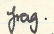
\includegraphics[width=.08\textwidth]{images/frag.png}};
    \node (m3image) [imageframe , right of=fragimage, xshift=.7cm] {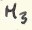
\includegraphics[width=.08\textwidth]{images/m3.png}};
    \node (azurelabel) [textcontainer, below of=imagelabel, yshift=.5cm] {OCR output};
    \node (frag) [textcontainer, right of=azurelabel, xshift=1cm] {frag.};
    \node (m3) [textcontainer, right of=frag, xshift=.7cm] {H3};
    \node (toothornot) [nnmodel, below of=frag, xshift=1.2cm, yshift=.5cm] {tooth or other?};
    \node (uplow) [nnmodel, below of=toothornot] {upper or lower?};
    \node (mpic) [nnmodel, below of=uplow] {M, P, I or C?};
    \node (mindex) [nnmodel, below of=mpic, xshift=-1.8cm] {1, 2 or 3?};
    \node (pindex) [nnmodel, below of=mpic, xshift=1.8cm] {1, 2, 3 or 4?};
    \node (end) [textcontainer, below of=mpic, yshift=-1.5cm] {frag. m3};

    \draw [arrow, draw=Blue] (2.9,-1.3) -- (toothornot);
    \draw [arrow] (m3) -- (toothornot);
    \draw [arrow] (toothornot) -- node[anchor=east] {tooth} (uplow);
    \draw [arrow] (uplow) -- node[anchor=east] {lower} (mpic);
    \draw [arrow] (mpic) --  node[anchor=east, yshift=0.2cm] {m} (mindex);
    \draw [nonactivearrow] (mpic) -- (pindex);
    \draw [arrow] (mindex) -- node[anchor=east, yshift=-0.2cm] {m3} (end);
    \draw [nonactivearrow] (pindex) -- (end);
    \draw[thick, draw=Blue] (1.9,-2) -- node[anchor=south] {other} (-1.7,-2) -- (-1.7,-8);
    \draw[->, thick, draw=Blue] (-1.7,-8) -- (2.7,-8);
    \draw[thick, draw=Maroon!30] (5.4,-5) -- (8.5,-5) -- (8.5,-8);
    \draw[->, thick, draw=Maroon!30] (8.5,-8) -- (4.7,-8);
\end{tikzpicture}

    \caption{Flowchart of the proposed tooth recognition pipeline}
    \label{fig:pipeline}
\end{figure}

For all words, bounding boxes, and reading results detected by Azure Vision on the element column, the word is first classified as tooth marking or other word.
To constrain the input data to the downstream model, this is completed 
with a regular expression checking whether the reading result of the word consists of a letter and number, or only the 
letter C. Once more robust classifiers are built, this part can be replaced with another deciding 
heuristic, allowing more variety in tooth-notation images to be cleaned. The regular expression 
only recognizes a small fraction due to frequent errors in bounding box detection.

The images of the words recognized as tooth markings are given to a binary image classifier deciding whether the tooth 
is upper or lower jaw and then to a model recognizing if the tooth type is molar, premolar, or incisor: as 
canines lack the number and are recognized as teeth only when the Azure Vision result is a letter C, there is 
no need to re-classify the tooth marking as a canine. It should be noted that as soon as the regular expression
heuristic is replaced with anything more complex, the fourth class has most likely to be added to the tooth type classifier.
Once the type is decided, the tooth marking image is given to the appropriate index number model. Finally, 
the three pieces of information obtained, jaw, type, and number, are combined as the digital tooth marking 
notation. As the final step, all words in the element column are concatenated, and all found teeth are 
collected as a tuple to the tooth records column.

To minimize required manual verification, additional confidence information is added 
to each tooth marking. As each classifier produces the probability of the image containing the 
chosen class as a side result, this probability can be saved as a confidence score. The confidence is taken 
per element description phrase (such as ``much of R. mandible ($\text{P}_4$ - $\text{M}_3$)'') by taking the minimum over all 
model confidence scores obtained during inference for the tooth records. For example, if in the 
example description, every other decision would be of 100\% confidence but the second tooth being a molar 
would only have 70\% confidence, the confidence of the entire row would be 70\%. This conservative approach is 
due to the costliness of errors: one needs to be absolutely certain before data can be left without manual 
verification.

Next, details related to building the classifiers presented in this section are specified.

\section{Building the models}
\label{sect:building-models}

For the dental marking recognition pipeline, four classifiers are needed: upper or lower jaw, 
tooth type, and two downstream index number classifiers. The experimental 
section considers design decisions for setting up experiments to build these models with maximal accuracy:
 Data preprocessing and augmentation along with base model,
transfer learning method and hyperparameter selection. After a presentation of how the training dataset was created, these aspects are considered.

\subsection{Creating the training dataset}

The dataset with a total of 1\,105 images was extracted from the fossil 
catalogues using the first two steps on the pipeline in Figure~\ref{fig:pipeline}:
for each word under the element-describing header, the Azure Vision output was classified 
to tooth or other with the regular expression, and 
images with tooth notation were cropped out from the catalogue. Along with the image, the 
Azure Vision \cite{azurevision} reading result was saved. To have as versatile notation as possible, images were 
extracted from several catalogues.

After extraction, data balancing, and splitting into training, testing, and validation sets 
was completed.
Because incisors and canines were much rarer 
than molars and premolars in the catalogues, some of the former were manually cropped out 
of catalogues to achieve more variety. After this, sample count differences 
 between the most frequent class and others were computed, and augmented 
images were saved for other classes to make sample counts per class equal. The augmentation 
was implemented using a random rotation of -5 to 5 degrees and a random crop with a scale from 0.9 to 1.0.
Train, validation, and test splits were selected by creating a validation dataset of roughly 200 samples to
 not change test error by more than 0.5\% with one sample classification
change. For the test set, 100 samples were kept. This resulted in 
train set sizes, including the images generated to balance classes, of 905 samples for upper or lower, 
2\,071 for M, P or I, 1\,521 for index one to three, and 2\,026 for index number one to four.

For data labeling, outputs from Azure Vision were heavily utilized. For 
tooth types and index numbers, if the reading result was a valid class, it was assumed to 
be correct and used as a label, saving a significant amount of labeling effort. As the 
images were saved in class-specific directories according to the PyTorch ImageFolder interface,
the correctness of labels could easily be verified by visual inspection. Upper and lower jaw labeling 
was completed manually with a ternary label, zero noting lower, one upper, and -1 an undecipherable jaw.
The undecipherable class was included as there were images where the jaw could not be decided by a human annotator, 
and therefore the correct answer for such an instance would be 'unknown'. Forcing these to be either upper or lower jaw 
would distort the classification task: perfect accuracy would be an undesirable result as the model should 
make mistakes with the undecipherable samples, and these would confuse the model as it is required to find signals on why 
the notation is either jaw when none are to be found. Therefore, images with undecipherable jaw were not given 
to the classifier.

As the work was completed under a non-disclosure agreement, the training datasets were not 
published. As the problem ended up being an interesting task from the perspective of optical character recognition, 
bringing even parts of the catalogue scans available for researchers and machine learning hobbyists is encouraged as it could prove
 valuable both for improving digitized data quality and advancing character recognition techniques.
 
A small sample of the training dataset of premolars is presented in Figure~\ref{image:samples}.

\begin{figure}[ht]
    \centering
    \includegraphics*[scale=.5]{images/trainingsamples.png}
    \caption{Samples from the training dataset for tooth type classification of premolar markings.}
    \label{image:samples}
\end{figure}

\subsection{Data preprocessing}
 
Preprocessing of training, validation, and test images was completed by grayscaling, denoising, and resizing.
As color channels in images have no meaning for the text on the image, grayscaling was implemented by
 stacking three identical grayscale images
to match the three-channel input size required by the base models.
Denoising was implemented due to
small paper texture shadow and eraser smudge noise with the most basic routine, a Gaussian filter.
The kernel size 3 was chosen by experimentation and visual inspection. Finally, the images were resized to 
ImageNet image size of 224x224 pixels using bilinear interpolation.
No further preprocessing was implemented to keep the images alike the source domain, ImageNet images with real-world noise.
 A catalogue sample before and after preprocessing can 
be found in Figure~\ref{image:noise}.

\begin{figure}[ht]
    \centering
    \resizebox{\linewidth}{!}{
        \begin{minipage}[b]{0.45\linewidth}
            \centering
            \includegraphics*[scale=0.67]{images/noise.png}
        \end{minipage}
        \hspace{0.5cm}
        \begin{minipage}[b]{0.45\linewidth}
            \centering
            \includegraphics*[scale=0.67]{images/denoised.png}
        \end{minipage}
    }
    \caption{A catalogue sample with paper texture shadow and eraser smudge noise before and after grayscaling and denoising.}
    \label{image:noise}
\end{figure}

More heavy preprocessing steps of binarization and extracting only the letter or number from the image were 
attempted but not implemented.
Binarizing the images was considered as evidence was found for binarization to increase result accuracy~\cite{9thuonPalm},
but was not implemented since the noise, in many cases
 parts of neighboring characters due to bounding box errors, are occasionally of darker 
color than the correct text, making thresholding difficult. Additionally,
 initial experiments with an MNIST base model suggested the resulting
accuracies were decreasing when using binary input images. However, the binarization scheme was not designed carefully 
and the experimentation was not exhaustive.
Another aspect considered after binarizing was to try to segment out the letter for the tooth type recognizer 
and the number to the index number recognizer, but it was found that there was so much variability 
among the images that implementing a deterministic algorithm was hard. 
As the premise of deep learning is that such challenging feature extraction becomes unnecessary as the neural 
network is better at extracting relevant information than a human designing preprocessing routines~\cite{princebook}, these 
heavier preprocessing operations were not used.

\subsection{Data augmentation}
\label{sect:aug}

Data augmentation operations were chosen according to variations that can 
occur among scans of documents with handwriting.
Due to paper and pen color differences, functions on pixel intensity
values were applied to adjust brightness and contrast by using the 
TorchVision ColorJitter transformation with brightness factor range from 
0.95 to 1.05 and contrast factor range from 0.8 to 1.2. To mimic bounding box detection errors, 
a random crop was implemented using RandomResizedCrop with 
scale from 0.9 to 1.0 to not crop out significant parts of the character but 
still introduce cropping variation. Rotation from -5 to 5 degrees 
was implemented as some tables were slightly tilted in the scan images. 
Lastly, handwriting variation was mimicked with horizontal and vertical 
shear by setting shear ranges for both horizontal and vertical directions from 1 
to 10 pixels with the RandomAffine operation. The background was filled in 
with white after rotation when necessary to match the other background as closely as possible.
 A batch of training images after augmentation
is presented in Figure~\ref{image:augmented}.

\begin{figure}[ht]
    \centering
    \includegraphics*[scale=.2]{images/augmented.png}
    \caption{Samples of the training dataset after data augmentation.}
    \label{image:augmented}
\end{figure}

\subsection{Base model selection}

To select appropriate base models, one first needs to select the source task and domain. Since most reviewed work uses image classification as the source task, this is assumed to work best.
Another potential source task would have been the identity mapping task given to the autoencoder,
but it was not implemented due to lesser popularity and the small size of the dental marking image dataset.
As the source domain, there are two datasets used in previous work: the classification of digits in the MNIST dataset, 
and the ILSVRC classification challenge with the ImageNet dataset. The popular 
assumption that ImageNet is a better source domain was verified with a short experiment by training an MNIST classifier~\cite{jamilemnist}
to classify tooth types with the best accuracy of 89\%, which was clearly outperformed by the ImageNet-based classifiers. This verifies the commonly assumed hypothesis that the domain of real-world images of any objects is a more 
similar one than the MNIST dataset of handwritten digits that is known to contain ideal-case images with little noise.

The ImageNet classifier base models used in the experiments are selected 
according to results from related work, reviewed in Section~\ref{sect:same_solution}.
The models were chosen by checking which base models 
occurred multiple times when listing the top three models in terms of accuracy. 
Analyzing Table~\ref{tab:model-info}, EfficientNet models~\cite{efficientnetv2} consistently outperform 
other architectures, most often with the V2S variant, closely followed by the 16-layer variant of the VGG architecture~\cite{vgg},
DenseNet121~\cite{densenet}, and ResNet101~\cite{resnet}.
Therefore, these four architectures were chosen as base models.
Additionally, the Vision Transformer~\cite{vit} and AlexNet~\cite{alexnet} were included, the former to test 
transformer architectures on the fossil domain and the latter
as proof-of-concept experiments suggested high accuracy scores.
The shortcoming in this base model selection is that as previous work did not give much
 reasoning for their base model selection, it is possible that some high-performing architectures were not included 
because they were not chosen to be experimented with. As one has to limit the 
search space of architectures in some way, previous success was kept as the main deciding heuristic 
even when acknowledging these limitations.

\subsection{Transfer method selection}

For transfer method selection, the reviewed work in Table~\ref{tab:model-info} has a variety of approaches, 
the only common trend being that freezing less seems to be beneficial. 
However, how much to freeze is dependent on transfer distance and target data size;
freezing more should work in cases similar as the features should be more useful 
and in cases of small target data, where overfitting is avoided.
For these reasons, it is argued that transfer method selection should be
based on experimentation rather than previous results.

For the choice of which layers to freeze, layers are only frozen so that a frozen layer never 
occurs after a trainable layer. This is because of the assumption that high-level layers 
encode generic and lower layers more specific features, and the generic features are assumed to be most transferable among tasks.
 Additionally, as specific features build on the generic ones, freezing layers 
below the ones modified is assumed to confuse the model. Therefore, all experiments consist of some layers 
at the start of the network being frozen and others at the end being open for updates.
The number of trained layers is used to specify the transfer method 
for each experiment, and these are always the last layers of the network.

As another experimentation principle, the trials start from settings where more layers are frozen, proceeding to
cases where more parameters can be updated. This is because more freezing saves 
computational effort, and is less likely to overfit to the training set as there is a lesser degree of freedom 
available for updating parameters. Therefore, it is sensible to look for a model that re-uses as 
many parameters as possible but still has enough flexibility to find a good optimum for the target problem:
This is assumed to result in the best generalization capability.

\subsection{Hyperparameter selection}

As for hyperparameters, values are selected according to well-performing 
options in reviewed literature to scope down the experimentation search space.
Hyperparameter tuning was not implemented to keep experimentation 
between approaches fair; if the optimization is better for some cases than others, one can no 
longer deduce whether the difference in result accuracy was due to hyperparameter or base model and 
transfer approach optimality. Therefore, hyperparameters are fixed between experiments to common values 
used previously in similar tasks. The selected hyperparameters, most chosen mostly by popularity 
with the only exceptions of reducing the number of epochs as experiments converged early
and adding learning rate scheduling to aid optimization,
are summarized in Table~\ref{table:hyperparameters}.

\begin{table}[h!]
    \centering
    \caption{Hyperparameters used in the experiments.}
    \begin{tabular}{ll}
    \hline
    \textbf{Hyperparameter} & \textbf{Value} \\ \hline
    Batch size & 64 \\ 
    Number of epochs & 20 \\
    Optimizer & Stochastic Gradient Descent with Momentum \\
    Momentum & 0.9 \\
    Learning rate & 0.001 \\
    Learning rate scheduler & Step (multiply by gamma=0.1 every 7 epochs)\\
    Loss function & Categorical cross-entropy \\ \hline
    \end{tabular}
    \label{table:hyperparameters}
\end{table}

In this chapter, the experimental setup along with reasoning for design decisions was given.
In the problem formulation, classifying words with a chain of univariate classifiers was opted for to 
maximize the accuracy by simplifying the problem as far as possible.
Preprocessing was kept minimal with denoising and grayscaling, 
and augmentation was set up according to variations that might occur in the scanning process. Base models were mostly
chosen according to previous success, resulting in the selection of the EfficientNetV2S, VGG16, DenseNet121, ResNet101, ViT, and AlexNet architectures.
Transfer methods are compared by experimentation: the model with most layers frozen while still being able to find a good optimum 
for the target task is searched for. In the next chapter, 
results from these experiments are presented and evaluated.

\chapter{Results and Discussion}

This chapter presents the results of the experiments. The base models were compared by
upper and lower jaw classification accuracy since initial experiments suggested it to be the most challenging task. The experimentation was limited to testing different base models, AlexNet, EfficientNetV2S, 
DenseNet121, Vision Transformer, and ResNet101, and freezing setups: training 1, 5, 10, or all layers.
The results of these experiments highlighted three major results. First, the best architectures were AlexNet and the Vision 
Transformer with best validation accuracies of 92.21 and 91.56, respectively, while EfficientNet performed poorly. Second, tests on changes in results 
when adjusting hyperparameters suggested that comparisons of model architectures should be taken with caution since one can never know 
if the differences in end accuracy were due to differences in model architecture or in how good the found optimum was. Lastly, as the strongest result, it is found that freezing less 
always increases result accuracy, and it is discussed whether this suggests that it is better to interpret transfer learning as extended 
training rather than a re-use of feature extraction. These aspects are discussed in more detail in this chapter. After this, future work suggestions are presented.

The experiment outcomes are collected in Table~\ref{table:results}, and 
the most important findings are the following. Using AlexNet as the base model results in the highest 
validation accuracy with the Vision Transformer as a close second. Having the transformer 
architecture not as the best but still a competitive accuracy verifies the result 
from Thuon et al.~\cite{9thuonPalm} that stated that convolutional networks outperform transformers, but suggests 
that transformer architectures are worth testing for in building various OCR
solutions. Another interesting point is that EfficientNet accuracies were the worst of all, 
which strongly contradicts the results of the reviewed works in Section~\ref{sect:same_solution},
suggesting that a model found to be better in one study can inform little on its performance in another target task.
The generalization capability of all models seems to be good, as seen in Figure~\ref{image:diff_hist}:
The difference between training and validation accuracies is in the majority of 
experiments below 4\%. As there is little correlation between the magnitude of this difference, 
a metric for the degree of overfitting, and layers trained, the initial hypothesis on freezing more to prevent overfitting
seemed to not hold.

\begin{table}[ht]
    \centering
        \scriptsize
        \begin{tabular}{|c|c|c|c|}
            \hline
            \textbf{Base Model} & \textbf{Layers Trained} & \textbf{Training Accuracy (\%)} & \textbf{Validation Accuracy (\%)}  \\ \hline
            AlexNet~\cite{alexnet}& all & 92.71 & $\mathbf{92.21}$       \\
            & 10 & 90.83 & 88.96          \\
             & 5    &84.30 & 80.52     \\
             & 1    & 64.09 & 61.69     \\\hline
             ViT ~\cite{vit}   & all  &95.25 & $\mathbf{91.56}$       \\
            & 10  & 68.84 & 66.88          \\
           & 5  & 68.73 & 64.94           \\
           & 1   &  50.06 & 42.86       \\\hline
           VGG16    ~\cite{vgg} & all  &90.72 & $\mathbf{87.01}$     \\
            & 10  & 84.31 & 80.52       \\
          & 5  &  72.27 & 67.53        \\
           & 1   &  43.65 & 35.06    \\\hline
          DenseNet121~\cite{densenet} & all  & 88.73 & 81.17   \\
            & 10  & 66.08 & 65.58  \\
           & 5  & 65.75 & 65.58   \\
           & 1   &  55.80 & 62.34   \\\hline
ResNet101 ~\cite{resnet}  & all  &            64.75 & 65.58  \\ 
           & 10  &  64.75 & 65.58    \\
           & 5  & 64.75 & 65.58   \\
          & 1   &   60.77 & 63.64  \\\hline
        EfficientNetV2S ~\cite{efficientnetv2}   & all  & 64.53 & 64.29   \\
            & 10  & 64.09 & 64.29    \\
           & 5  & 64.09 & 64.29  \\
          & 1   &   54.59 & 54.55  \\\hline
        \end{tabular}
    \caption{Training and validation accuracy for different base models and layer freezing setups for upper or lower jaw classification}
    \label{table:results}
\end{table}

\begin{figure}[ht]
    \centering
    \includegraphics*[scale=0.7]{images/train_val_error_difference_histogram.png}
    \caption{Histogram of percentage-point differences in training and validation accuracies within each experiment}
    \label{image:diff_hist}
\end{figure}

To estimate how much the results depended on the optimum found in training and how much on the architecture, 
the best architecture AlexNet was retrained with one hyperparameter changed. The resulting 
change in accuracy suggests that comparing architectures when target data is small is highly inaccurate. 
A change in the random seed from 15 to 2, both randomly chosen, was done to check how much the result changes 
when the only thing that changed is the order of training samples in batches. This changes which initial examples are shown to the model,
changing the initial steps of the learning trajectory, which is important in neural network training~\cite{transferlearning_survey}.
 As seen in Table~\ref{table:random_seed_sensitivity}, the largest difference occurred with one layer 
trained, and the second seed had the validation accuracy increased by 9.09 percentage points. This shows that initial examples 
are important and can initialize much better or worse learning trajectories. Then, hyperparameter change 
by changing batch size from 64 to 32, also a random choice, was tested with the AlexNet architecture, and the results 
changed by at most 6.49\%, as seen in Table~\ref{table:hyperparameter_sensitivity}. Notably, the best accuracy was outperformed by as much as 4.54 percentage points 
in this setting, more than halving the count of errors. These large variances serve as a good example of the caveats of comparing 
base models in a small data setting: since there is no objective metric for the quality of an optimum, there 
is practically no way of knowing what the true reason for accuracy differences between experiments is. In this case, the 
margin of error can be approximated at 10\%, that is, only when validation accuracies differ by more than that one can be 
somewhat confident that the better result actually has a superior architecture. Taking this into account, AlexNet, ViT, and VGG16 
can all be considered best-performing architectures in this study. Having access to more validation data or more computational 
resources to repeat the experiments with different hyperparameter settings would be required to draw more fine-grained conclusions on the 
superiority of one architecture over another.

\begin{table}[ht]
    \centering
        \scriptsize
        \begin{tabular}{|c|c|c|c|}
            \hline
            \textbf{Accuracy, first seed (\%)} & \textbf{Accuracy, second seed (\%)} & \textbf{Difference (\%)} & \textbf{Layers Trained} \\ \hline
            88.31 & 92.21 & 3.90  & all \\\hline
            85.71 & 88.96 & 3.25 & 10  \\\hline
            75.32 & 80.52 & 5.20  & 5   \\\hline
            52.60 & 61.69 & 9.09 & 1   \\\hline
        \end{tabular}
    \caption{Random seed sensitivity: validation accuracies with two different seed values}
    \label{table:random_seed_sensitivity}
\end{table}

\begin{table}[ht]
    \centering
        \scriptsize
        \begin{tabular}{|c|c|c|c|}
            \hline
            \textbf{Accuracy, batch size 64 (\%)} & \textbf{Accuracy, batch size 32 (\%)} & \textbf{Difference} (\%) & \textbf{Layers Trained} \\ \hline
            92.21 & 96.75 & 4.54 & all \\\hline
            88.96 & 93.51 & 4.55 & 10  \\\hline
            80.52 & 87.01 & 6.49 & 5   \\\hline
            61.69 & 61.69 & 0.00 & 1   \\\hline
        \end{tabular}
    \caption{Hyperparameter sensitivity: validation accuracies with batch sizes 64 and 32}
    \label{table:hyperparameter_sensitivity}
\end{table}

The clearest result from the experiments is that freezing never improved the resulting accuracy. This result was 
also the only larger consensus among studies reviewed in Section~\ref{sect:same_solution}.
As is highlighted in the plot of layers trained against resulting accuracy in Figure~\ref{image:accuracy_vs_freezing},
there were no exceptions to this relationship. The accuracy of DenseNet121 and ResNet101 plateauing can be seen as 
the model having enough freedom to encode all information present in the training data and therefore adding 
more trainable parameters did not increase accuracy. To interpret the correlation, the hypothesis that using a feature 
extractor as is, inspired by the Tibetan glyph classification solution~\cite{4zhaoTibetan}, did not result in the 
best model in the fossil domain; additional feature tuning was needed.

\begin{figure}[ht]
    \centering
    \includegraphics*[scale=0.8]{images/accuracy_against_freezing.png}
    \caption{Line plots of accuracy scores with different freezing setups reveal the positive correlation of accuracy and count of layers trained.}
    \label{image:accuracy_vs_freezing}
\end{figure}

To analyze transfer distances, less rigorous experiments were implemented on an MNIST base model~\cite{jamilemnist}.
This was implemented to check the hypothesis that the transfer distance from MNIST to fossil data is larger than that where 
the base task is ImageNet: even though the former contains characters, the ideal-case benchmark images are more dissimilar 
as they contain no clutter or noise prominent in real-world images~\cite{alexnet}. This was found to be true; 
initial experimentation, although not as rigorous as the ImageNet-based experiments, never achieved above-90\% accuracies.
This result was shared by the handwritten Gujarati detection study~\cite{8goelGujarati2023}, where ImageNet as the base task 
outperformed MNIST in all layer-freezing scenarios. 

To draw an analogue from neural networks to learning in general, the central lesson learned in these experiments 
is that there is no trickery to learning. To learn something, there are two avenues: one is to learn principles, which in 
neural networks occurs by encoding prior information with architectures or constraining the problem space. After that, the only 
option is to repeatably expose the learner to examples. The feature-recycling premise of transfer learning seems to be that 
by reusing features, some of this example study could be circumvented. That freezing less never deteriorated performance
raises the hypothesis that this could be untrue, that the real value of transfer learning is that a part of the learning from 
examples is re-used from another training run, allowing for training longer and therefore seeing more examples. Transfer distance 
fits in this with the intuition that all examples seen to learn a trend need to be relevant to the problem. 
Taking the idea that transfer utility is only about 
seeing more examples further, one can even hypothesize whether the superiority of ImageNet over other base tasks, like MNIST, is 
due to the transfer distance being shorter or if the reason is the sheer size of the dataset. Summarizing all this, the lesson learned
can be boiled down to one phrase, much alike the GoogLeNet inspiring meme~\cite{we_need_to_go_deeper}: one can say ``we need to go further'', that the way forward is only about exposing the model to more examples, 
and re-using the previously learned as much as possible.

Returning to the higher-level task of correcting dental markings, all models presented in Section~\ref{sect:pipeline} were constructed, evaluated, and used 
in building the inference pipeline. For evaluation, test error was measured on a new set not used in previous experiments 
to prevent data leakage; data used to inform the model-building process should never be used to report final accuracies~\cite{engbook}.
A certainty score was constructed to measure what fraction of images was classified with above-human accuracy of 99,7\% to measure 
how much manual verifying labor can be saved with the system. The evaluation results are presented in Table~\ref{tab:task_accuracy_certainty}.
The results align with intuition from the labeling process; labeling images 
where Azure Vision~\cite{azurevision} had made a mistake felt easiest 
with the letter and hardest for the number, largely due to bounding box errors 
cutting off parts of the digit. Often, the bottom was cut off, causing digits two and three to become indistinguishable. Also judging on the labeling experience,
the results with custom-made models outperform the generalist, although no 
correctness metrics were counted for the Azure Vision readings. 
As for limitations for these results, results need to 
be taken with caution as varying the random seed caused fluctuations of 
up to 10\% also in evaluation. The test accuracies can also be inaccurate because 
of severe class imbalance, especially for the index numbers, where the digit 1 was so few
that the model may have overfit to these examples.
Finally, as seen in Figure~\ref{image:misclassifications_uplow_in_test},
the upper and lower jaw classifier struggled to classify canines correctly;
only seven instances like these were present in the test set, five of 
which were misclassified. On the other hand, this also means that other upper 
and lower jaw classifications were learned well. This is suggested by 
the pipeline outcomes: all images tested, albeit a small sample, were 
assigned a correct dental marking. In the aggregated confidence score, 
high individual subtask confidences were undermined by some lower confidences, 
causing most of the final confidence scores to be below human-level accuracy, leading 
to possibly only a small amount of saved manual verifying effort. 
A snapshot of dental markings constructed can be seen in Figure \ref{image:inference}.


\begin{table}[h!]
\centering
\begin{tabular}{|l|c|c|}
\hline
\textbf{Task}       & \textbf{Accuracy (\%)} & \textbf{Certainty (\%)} \\ \hline
M, P, I                 & 100.00                 & 94.50                   \\ \hline
Upper, Lower         & 92.31                  & 71.79                   \\ \hline
Index (1-3)                 & 88.00                  & 58.00                    \\ \hline
Index (1-4)                & 91.39                  & 62.92                   \\ \hline
\end{tabular}
\caption{Test accuracy and certainty levels. Certainty measures the fraction of examples recognized with above-99.7\% confidence.}
\label{tab:task_accuracy_certainty}
\end{table}

\begin{figure}[ht]
    \centering
    \includegraphics*[scale=0.8]{images/misclassified_uplow.png}
    \caption{All misclassified samples from the upper or lower jaw test set. The letter C with a line on top or bottom is detected poorly; seven of these were present in the test set.}
    \label{image:misclassifications_uplow_in_test}
\end{figure}

\begin{figure}[ht]
    \centering
    \includegraphics*[scale=0.8]{images/inference.png}
    \caption{Sample outputs of dental notation and associated confidence values. Only few of the samples exceed human-level classification accuracy of 99,7\%.}
    \label{image:inference}
\end{figure}

\section{Future work on digitizing fossil catalogues}

While this work managed to accurately clean a part of dental markings present in the catalogues, 
there are several potential directions to significantly improve the digitization of such catalogues in general, the main direction 
being improving the quality of word-location defining bounding boxes. The main problem in the bounding boxes provided 
by Azure Vision~\cite{azurevision} was that the dental marking words were often cut across many words or were present 
as a part of a longer word. This is likely due to the space width varying greatly between different pieces of 
handwriting, and sub- or superscripts being unfamiliar to the model. To improve the correctness of handwriting segmentation, developing a fine-tuned word detector 
could improve the result: a specialist model encoded with knowledge of what kinds of words are more likely to be 
present in the data would likely be better at finding a correct segmentation. An example of 
such case is seen in Figure~\ref{image:hardsentence}: a segmenter with the knowledge of tooth marking notation could 
easily see that the $\text{dm}_{3-4}$ section is one word, which is difficult to a generalist model 
due to the spacing between characters.

\begin{figure}[ht]
    \centering
    \includegraphics*[scale=0.8]{images/hardwordsegmentation.png}
    \caption{Example of a sentence hard to segment to words without context knowledge.}
    \label{image:hardsentence}
\end{figure}

The problem of finding objects in images is much harder than image classification and has attracted attention 
from the computer vision research community recently\footnote{These were surveyed at the lecture ``Computer Vision Applications with CNNs'' on the course Computer Vision, presented at the University of Helsinki, Faculty of Science by professor Laura Ruotsalainen on 11th October 2024.}. 
The main reasons for the difficulty are the labor required to obtain ground truth bounding boxes and object detection requiring better image resolution to work well, therefore requiring more computational resources.
One way to circumvent manual annotation for fossil catalogues could be to automatically detect correct bounding boxes 
from commercial OCR engine outputs, for instance by regular expression matching the word readings with a vocabulary of words likely to be 
present in fossil catalogues, much like the approach implemented in this work.
For the segmentation model, several recent advances seem promising, but might not be directly applicable without fine-tuning 
due to the standard problem of object detection being the detection of three-dimensional objects in scenes,
quite a different problem from word detection on a flat, scanned document. This is likely the reason an initial experiment 
ran on the Hugging Face API version~\cite{OmouredYOLOv10DocumentLayoutAnalysisHugging2023} of YOLO-10~\cite{wang2024yolov10}, a variant of the highly influential object detector YOLO~\cite{redmonYouOnlyLook2016},
resulted in a poor segmentation found in Figure~\ref{image:yolo}: the entire image was segmented as one object.
Some possibly more applicable models, however not as easily testable due to lesser popularity, 
are the open-vocabulary version of YOLO~\cite{YOLOWorldRealTimeOpenVocabulary},
 the hierarchical text spotter~\cite{longHierarchicalTextSpotter2024}, and the Detectron from Meta~\cite{Detectron}.
 However, due to the catalogue-specific problem illustrated in Figure~\ref{image:hardsentence}, these 
 models would likely require well-optimized fine-tuning to work. It is also possible that the transfer distance from a three-dimensional scene to a scan image is 
 too large and OCR-specific object detectors need to be found. Experimenting with such implementations is a 
 substantial effort and was omitted from this work to keep the scope reasonable.

Another possible line of extending the work would be improving the accuracy of the dental marking classification. 
Some ideas include to extend the model with capabilities of detecting markings with multiple teeth,
a rather unusual case of multi-class character classification, and to experiment with more recent ImageNet classifiers with better top-5 and top-1 error rates.
However, using the newer models would require more effort since good pre-trained weights are 
more difficult to find for the less established models, and there is less evidence of their applicability to downstream tasks. Improving the model would still be useful, since a more sophisticated word segmenter would result in a more 
variable set of tooth marking images to be given to the classifiers, making the classification problems more difficult. 
Still, the object detection problem should be given more attention since even the 
potential harder variants of the dental marking classification task are relatively simple image classification problems when comparing 
them to challenges such as basic ImageNet classification.

\begin{figure}[ht]
    \centering
    \includegraphics*[scale=0.29]{images/yoloresult.png}
    \caption{Preliminary object detection test with the YOLO-10 object detector using the Hugging Face inference API~\cite{OmouredYOLOv10DocumentLayoutAnalysisHugging2023}.}
    \label{image:yolo}
\end{figure}

\chapter{Conclusions}

Returning from the problem of digitizing handwritten fossil specimens to the larger picture, several thoughts arose on the potential of centralized, structured databases for paleontological research from short conversations with practitioners.
These ideas can be viewed as a reiteration of what was attempted in this thesis, or toward which goal a tiny step was made. For any large endeavor one needs a guiding goal to inform the direction of developing methods, and looking from a data management perspective, it seems that the best-case goal for paleontological databases is obtainable and holds a large potential for avoiding routine work for more meaningful activities. To conclude this work, these ideas are explored: what could be possible, what the utility of such advancements would be, what has been already done within these domains, and what further work is required to achieve the goals.

To see what could be, a good analogue to start from is that of scientific journals. If those were what fossil data largely is like today, journals would be scattered around the world, some saved digitally, some in paper form. Should someone want to study a subject, the work would start from finding where interesting material could reside, traveling to the location, and saving photocopies of physical and copies of digital work. The best-case future scenario for fossil data would be like Google Scholar is for research: one search box, where a researcher wishing to analyze a subject could write, for instance, ``all lower third molars globally, with all loph counts, dated and with location'' using some query language, and a dataset could be created in seconds. With a multimodal database, 3D images of the physical samples could be stored along with each data entry. Setting specific features aside, the main premise is that the technological tools for creating an all-encompassing dataset are not utopian and that it is possible to dramatically increase the efficiency of data acquisition.

The Google Scholar analogue likely highlighted already what the utility of a global, all-encompassing paleontological database could be, but several more benefits should be covered. To state the obvious, huge amounts of tedious data acquisition and uniforming effort could be saved, and this saved time could then be spent conducting more research, thinking deeply about the analytical problems, or not working at all. Another type of work that could be saved significantly is that of data creation: if every measurement and taxon identification, after completion, could be saved indefinitely and for everyone to access, no measuring would be done twice. Additionally, when saving new measurements, the result tractability could be improved with metadata: the person completing the measurement, the date, and any thoughts regarding the measurement could be saved. Should any doubts of the correctness of a measure or taxon identification arise, this data or the person could be consulted, and the entry corrected if necessary. Versioning schemes could be designed to save a history of these corrections. Should one want to see the physical samples, the database still had an utility of serving as a search engine for finding where relevant specimens reside. Lastly, this much more standardized approach to fossil data would allow much better reproducibility: the database query to get the dataset used in each study could be published, and the data could be obtained by anyone evaluating the study to re-run or further experiment with the analysis conducted. With these changes in habits of data management, the thing that matters, quality of knowledge of the distant past, could be dramatically improved.

The automated correction of tooth markings implemented in this thesis can be viewed as a small step toward this goal. The most positive outcome was that the tooth type letter classification achieved perfect 100\% accuracy, most likely due to its dominant position in the dental marking images. More challenging turned out to be comparing different base models, due to large fluctuations in results with hyperparameter changes; and index number detection, due to bounding box errors and the less dominant position of the digit in the image. The largest limitation found was the quality of the word bounding boxes: the generalist segmentation algorithm had challenges with segmenting the tooth markings, which could be improved by creating a fine-tuned character segmentation model. The most important finding of all, however, was that automated correction of fossil data is a fairly unresearched area and that much remains to be done until reliable enough pipelines to bypass human supervision can be built. Therefore, it is encouraged that the first focus should be on the establishment of good data management practices for the data already available digitally, as this is the best way to save work in data acquisition and with that improve paleoecological research. This also allows the data digitized later to be saved in an easily accessible format, which is a prerequisite for automated digitization to be of practical use.

What it would take to progress from the current state of the art is mostly to continue work already underway, by standardizing and increasing the size of globally available structured data.
For digitizing, when comparing to traditional annotation by hand, automated digitization holds potential by being able to increase the capacity of data creation, although the challenge remains that perfect correctness is needed to avoid manual verification. However, as seen in this thesis, the accuracies achieved with well-established character recognition methods seem promising.
To unify data formats, standards of measurement are required: what should be measured, and in which units. For these, standardization projects such as Darwin Core~\cite{darwincore} or the Ecological Trait-data Standard~\cite{ets-trait-data-standard} are well-established, but conforming to these standards is not universal~\cite{groomImprovedStandardizationTranscribed2019}.
Lastly, one of the main efforts is to collect data, for which several ambitious projects with a long history, such as the GBIF repository~\cite{gbif}, exist.
 Still, what is required is an incentive to contribute to global databases: after 
conducting an analysis, undergoing the additional effort of sending out the measurements is currently not required. As is known by all natural scientists, species that collaborate flourish, and it is in the interest of everyone to do what one can to advance the whole field.

\chapter{Acknowledgements}

I am sending thanks to the following people for help with the thesis process.
To my supervisor Professor Indr{\.e} \v{Z}liobait{\.e}, for quick replies to messages, the invitations to group meetings, and help with most relevant research aspects rather than overfocusing on presentation style.
To PhD Kari Lintulaakso from LUOMUS, for acting as the spring project contact, helping with forming the thesis topic, and several comment rounds on the work.
To ICT Officer Stephen Maikweki from the National Museums of Kenya for making the whole project possible by initiating the digitization effort and completing the most laborious part of the whole: scanning the 4\,200 pages of catalogues and numerable specimen cards, and taking the time to meet us to while visiting Finland.
To the Data Science Project group, Max V\"{a}ist\"{o}, Axel Wester, Yinong Li, and Janne Tuukkanen for the successful project that made this thesis topic possible: implementing digitization to an extent after which building one's own OCR engine was a sensible next step to do. Additionally, the reusable coding style saved hours of programming in experimentation for the thesis.
To Emeritus Professor Mikael Fortelius for showing interest in my work, shedding light on the significance of advancing automated data curation for paleontological data, and giving ideas on what the reasons for the lack of research in paleontological data management might be.
To PhD student Shayan Gharib for serving as an ad-hoc research tutor by email; the help with code errors I was blind to and understanding new concepts was of great aid at the start of the work.
To the Kurt\'{e}n club members, for the welcoming attitude and symposium invitation that allowed me to talk to people more freely and get a better impression of what the practicalities of doing paleontological analysis are like.
%Lastly, for final comments and proofreading help, thanks to.

\cleardoublepage
\phantomsection

\addcontentsline{toc}{chapter}{\bibname}
\bibliographystyle{abbrv}
\bibliography{bibliography}

\end{document}